\documentclass[aspectratio=169]{beamer}

\usepackage[T5]{fontenc}
\usepackage[utf8]{inputenc}
\usepackage{lmodern}

\usetheme{Madrid}

\usepackage{graphicx}
\usepackage{multicol}
\usepackage{amsmath,amssymb}

% Outline look: blue text, numbered, no balls
\setbeamertemplate{section in toc}{%
  \leavevmode\inserttocsectionnumber.~\inserttocsection\par}
\setbeamercolor{section in toc}{fg=blue}

\hypersetup{colorlinks=true, urlcolor=blue}

\newcommand{\backbtn}{%
  \hfill\hyperlink{outline}{\beamerbutton{Mục lục}}}


% Giảm khoảng cách trên/dưới công thức hiển thị để slide gọn hơn
\makeatletter
\def\tight@disp{\setlength\abovedisplayskip{4pt plus 2pt}%
  \setlength\belowdisplayskip{4pt plus 2pt}%
  \setlength\abovedisplayshortskip{2pt plus 1pt}%
  \setlength\belowdisplayshortskip{2pt plus 1pt}}
\g@addto@macro\normalsize{\tight@disp}
\g@addto@macro\small{\tight@disp}
\g@addto@macro\footnotesize{\tight@disp}
\g@addto@macro\scriptsize{\tight@disp}
\makeatother

\title[Độ võng của dầm]{Độ võng của dầm}
\author[© N. V. Sỹ]{Nguyễn Văn Sỹ}
\institute[TNUT]{%
  Bộ môn Hệ thống Công nghiệp \\
  Trường Đại học Kỹ thuật Công nghiệp \\
  \href{mailto:vansy@tnut.edu.vn}{vansy@tnut.edu.vn}}
\date[Cơ học vật liệu]{\large Cơ học vật liệu – Độ võng của dầm \\[0.5em] \footnotesize \copyright\ Nguyễn Văn Sỹ}

\begin{document}

\begin{frame}
  \titlepage
\end{frame}
%====================
\begin{frame}{Tài liệu tham khảo}
	\small
	F. P. Beer, E. R. Johnston, Jr., J. T. DeWolf, D. F. Mazurek,
	\emph{Mechanics of Materials}, 6th ed., McGraw-Hill, New York, 2012.
	
	\vspace{1em}
	\footnotesize\color{gray}
	Toàn bộ hình vẽ trong bài giảng được trích từ giáo trình trên, chỉ sử dụng
	cho mục đích giảng dạy nội bộ.
\end{frame}
% ===== OUTLINE SLIDE =====
\begin{frame}[t]{Nội dung}
  \hypertarget{outline}{}
  \tiny
  \begin{multicols}{2}
    \tableofcontents[hideallsubsections]
  \end{multicols}
\end{frame}

% ===== CONTENT SLIDES =====
\section{Biến dạng của dầm chịu tải trọng ngang}
\begin{frame}[t]{Biến dạng của dầm chịu tải trọng ngang}
  \begin{columns}[T]
    \column{0.58\textwidth}
      \small
      \begin{itemize}
        \setlength{\itemsep}{0.5em}
        \item Quan hệ giữa mô men uốn và độ cong khi uốn thuần túy vẫn đúng
              cho trường hợp tải trọng ngang tổng quát:
        \[
          \frac{1}{\rho} = \frac{M(x)}{EI}
        \]
        \item Dầm công xôn chịu lực tập trung ở đầu tự do:
        \[
          \frac{1}{\rho} = -\frac{Px}{EI}
        \]
        \item Độ cong thay đổi tuyến tính theo $x$.
        \item Tại đầu tự do $A$: \quad
              $\dfrac{1}{\rho_A} = 0$, \quad $\rho_A = \infty$
        \item Tại ngàm $B$: \quad
              $\dfrac{1}{\rho_B} \neq 0$, \quad $\rho_B = \dfrac{EI}{PL}$
      \end{itemize}
    \column{0.40\textwidth}
      \centering
      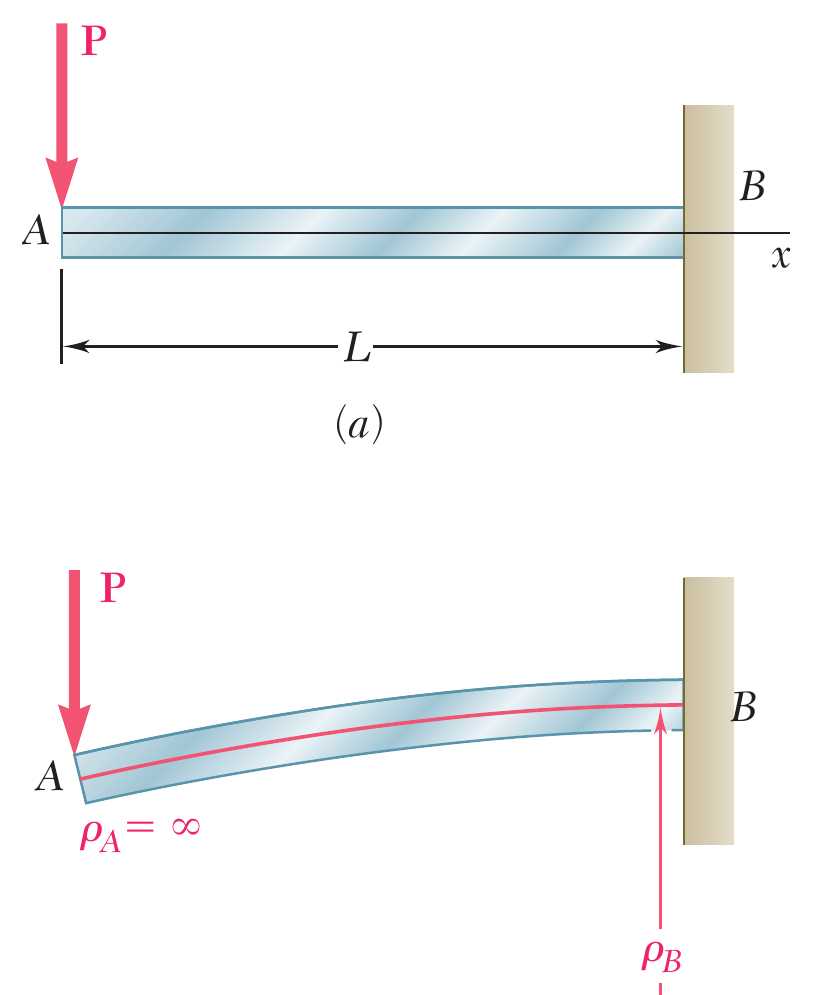
\includegraphics[width=\linewidth,height=5.5cm,keepaspectratio]{Chap_9/fig_9_3.png}
  \end{columns}
\end{frame}
% ===========
\begin{frame}[t]{Biến dạng của dầm chịu tải trọng ngang (tiếp)}
  \begin{columns}[T]
    \column{0.58\textwidth}
      \footnotesize
      \begin{itemize}
        \setlength{\itemsep}{0.17em}
        \item Dầm có đầu thừa.
        \item Phản lực tại $A$ và $C$.
        \item Biểu đồ mô men uốn.
        \item Độ cong bằng không tại các điểm có mô men uốn bằng không, tức là
              tại hai đầu và tại $E$:
        \[
          \frac{1}{\rho} = \frac{M(x)}{EI}
        \]
        \item Dầm võng lõm lên trên ở đoạn mô men uốn dương và lõm xuống dưới
              ở đoạn mô men uốn âm.
        \item Độ cong lớn nhất xuất hiện tại nơi trị tuyệt đối của mô men lớn
              nhất.
        \item Cần có phương trình hình dạng dầm, hay \emph{đường đàn hồi}, để
              xác định độ võng và góc xoay lớn nhất.
      \end{itemize}
    \column{0.40\textwidth}
      \centering
      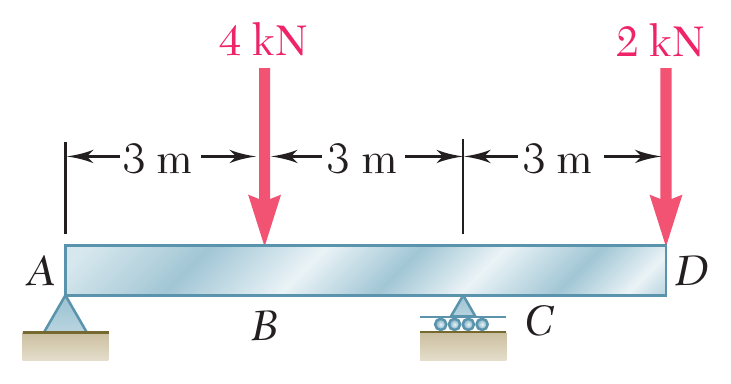
\includegraphics[width=\linewidth,height=1.6cm,keepaspectratio]{Chap_9/fig_9_4_a.png}\\[2pt]
      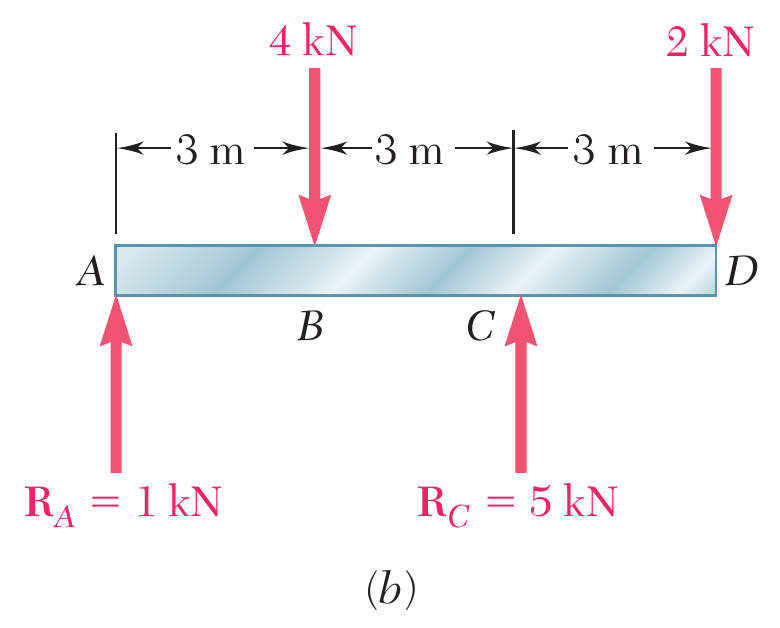
\includegraphics[width=\linewidth,height=1.6cm,keepaspectratio]{Chap_9/fig_9_4_reactions.png}\\[2pt]
      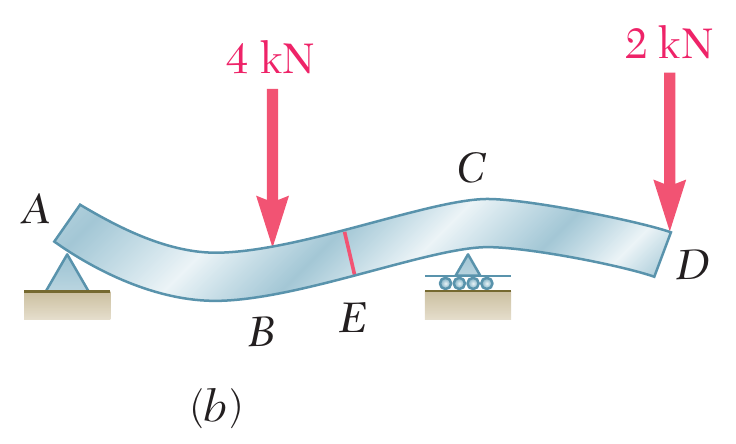
\includegraphics[width=\linewidth,height=1.6cm,keepaspectratio]{Chap_9/fig_9_4_b.png}
  \end{columns}
\end{frame}
% ===========
\section{Phương trình đường đàn hồi}
\begin{frame}[t]{Phương trình đường đàn hồi}
  \begin{columns}[T]
    \column{0.58\textwidth}
      \small
      \begin{itemize}
        \setlength{\itemsep}{0.6em}
        \item Từ giải tích, đơn giản hóa cho các thông số của dầm:
        \[
          \frac{1}{\rho} = \frac{\dfrac{d^2y}{dx^2}}
            {\left[1 + \left(\dfrac{dy}{dx}\right)^2\right]^{3/2}}
          \approx \frac{d^2y}{dx^2}
        \]
        \item Thay vào và tích phân:
        \[
          EI\frac{1}{\rho} = EI\frac{d^2y}{dx^2} = M(x)
        \]
        \[
          EI\theta \approx EI\frac{dy}{dx} = \int_0^x M(x)\,dx + C_1
        \]
        \[
          EI\,y = \int_0^x dx\int_0^x M(x)\,dx + C_1x + C_2
        \]
      \end{itemize}
    \column{0.40\textwidth}
      \centering
      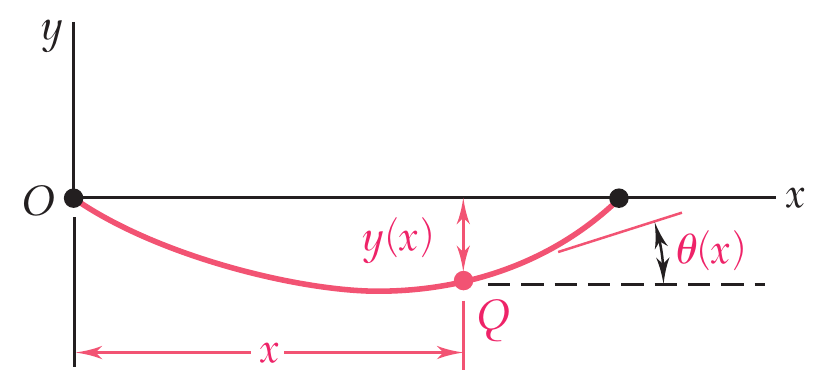
\includegraphics[width=\linewidth,height=5.5cm,keepaspectratio]{Chap_9/fig_9_7.png}
  \end{columns}
\end{frame}
% ===========
\begin{frame}[t]{Phương trình đường đàn hồi (tiếp)}
  \begin{columns}[T]
    \column{0.58\textwidth}
      \small
      \begin{itemize}
        \setlength{\itemsep}{0.5em}
        \item Các hằng số được xác định từ điều kiện biên:
        \[
          EI\,y = \int_0^x dx\int_0^x M(x)\,dx + C_1x + C_2
        \]
        \item Ba trường hợp đối với dầm tĩnh định:
              \begin{itemize}
                \item Dầm tựa đơn: \quad $y_A = 0$, \ $y_B = 0$
                \item Dầm có đầu thừa: \quad $y_A = 0$, \ $y_B = 0$
                \item Dầm công xôn: \quad $y_A = 0$, \ $\theta_A = 0$
              \end{itemize}
        \item Các tải trọng phức tạp hơn đòi hỏi nhiều tích phân và áp dụng
              điều kiện liên tục của chuyển vị và góc xoay.
      \end{itemize}
    \column{0.40\textwidth}
      \centering
      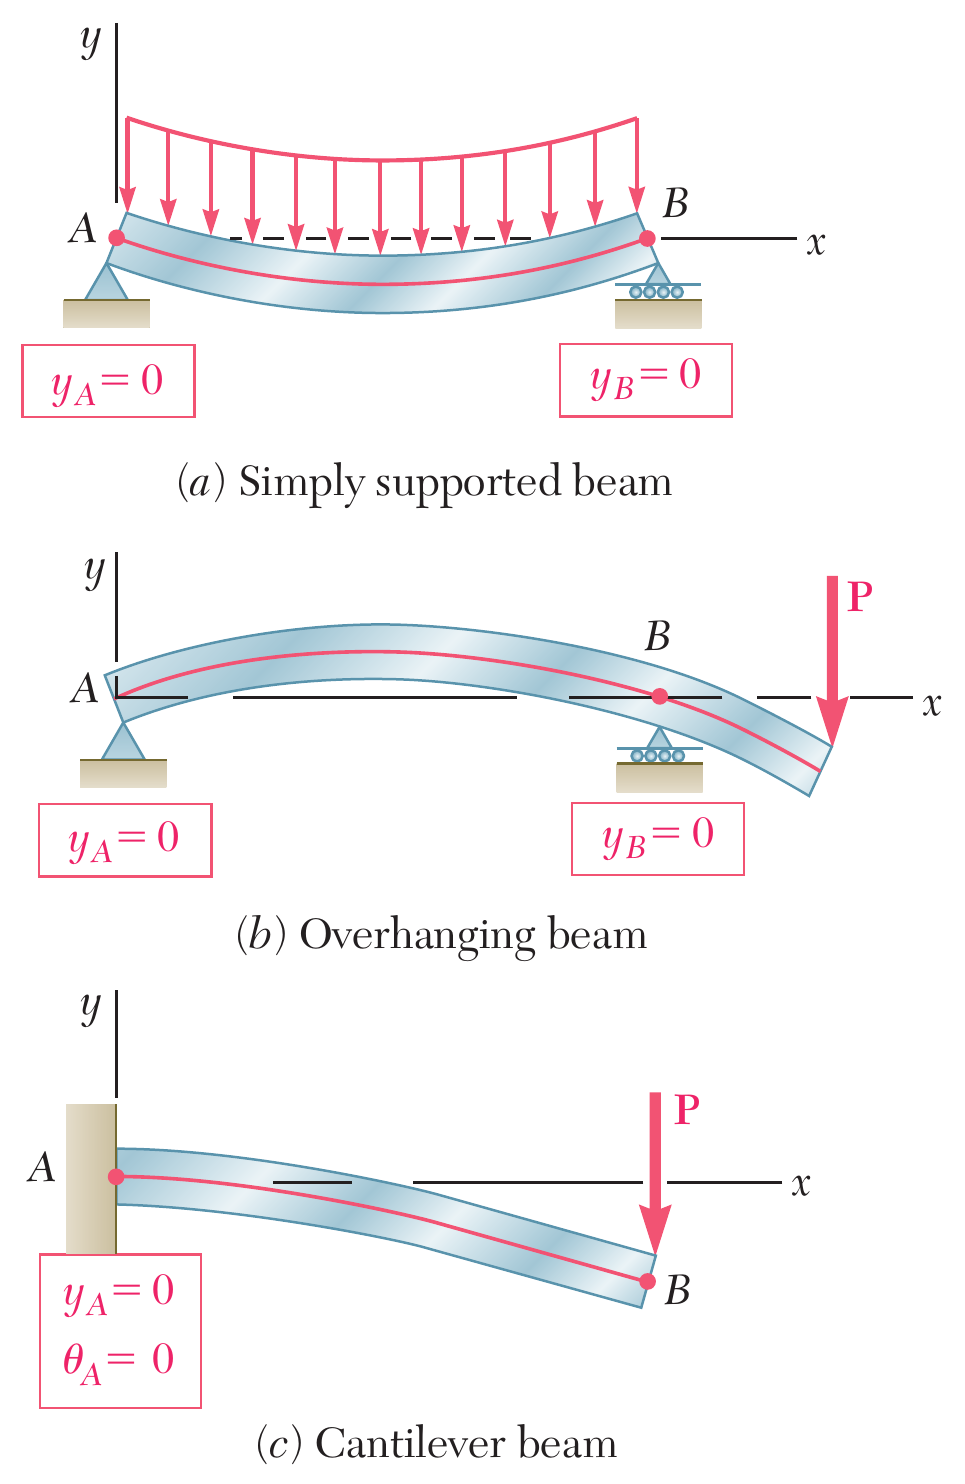
\includegraphics[width=\linewidth,height=1.9cm,keepaspectratio]{Chap_9/fig_9_8.png}\\[2pt]
      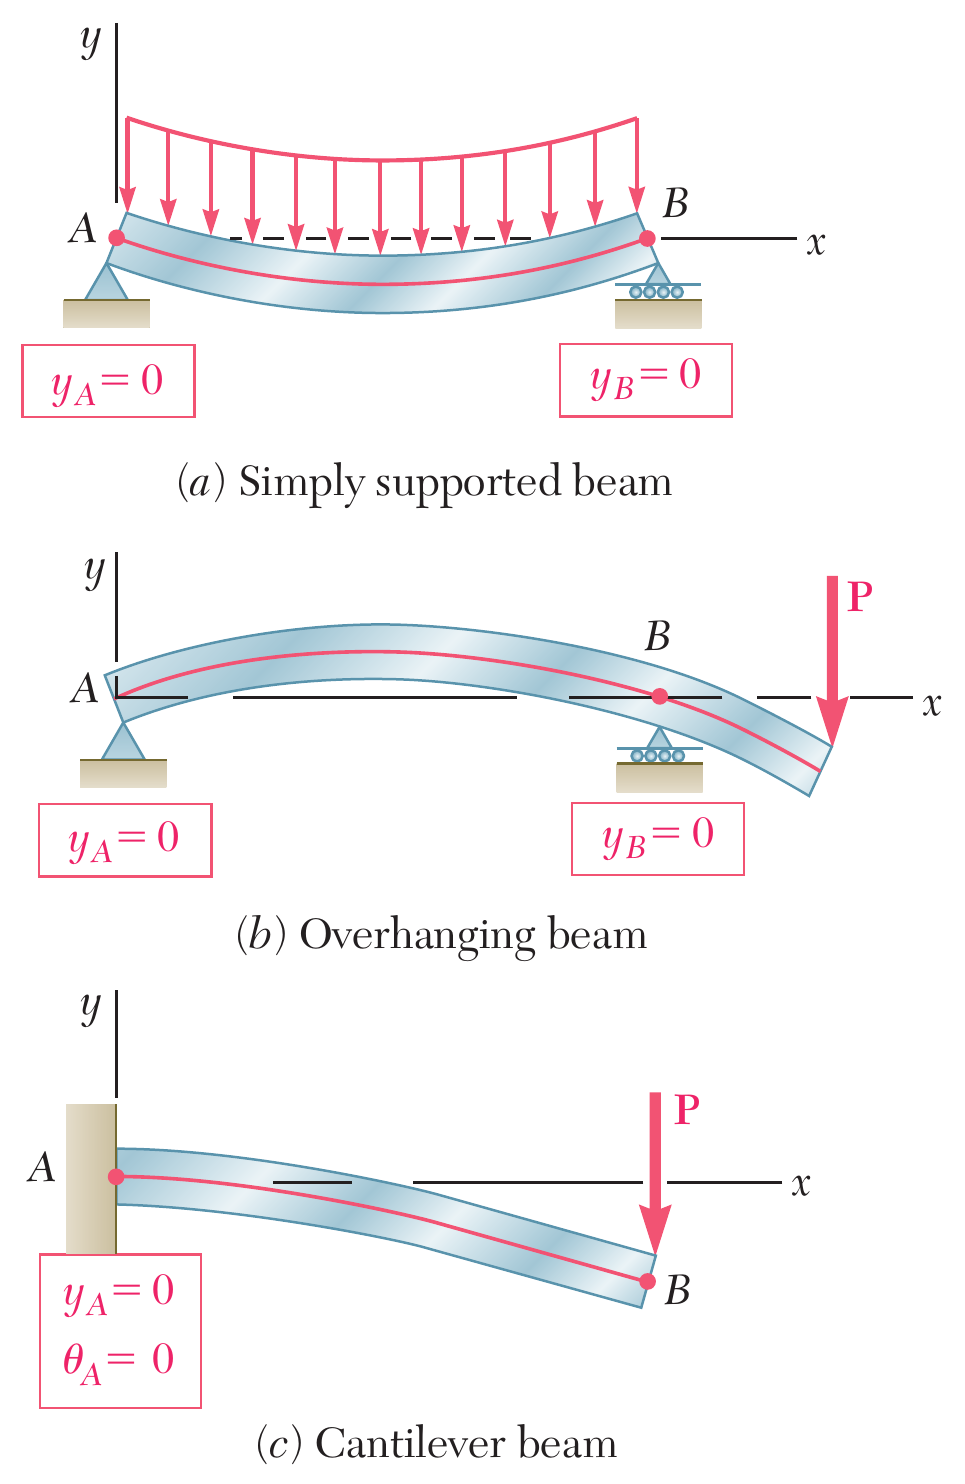
\includegraphics[width=\linewidth,height=1.9cm,keepaspectratio]{Chap_9/fig_9_8.png}\\[2pt]
      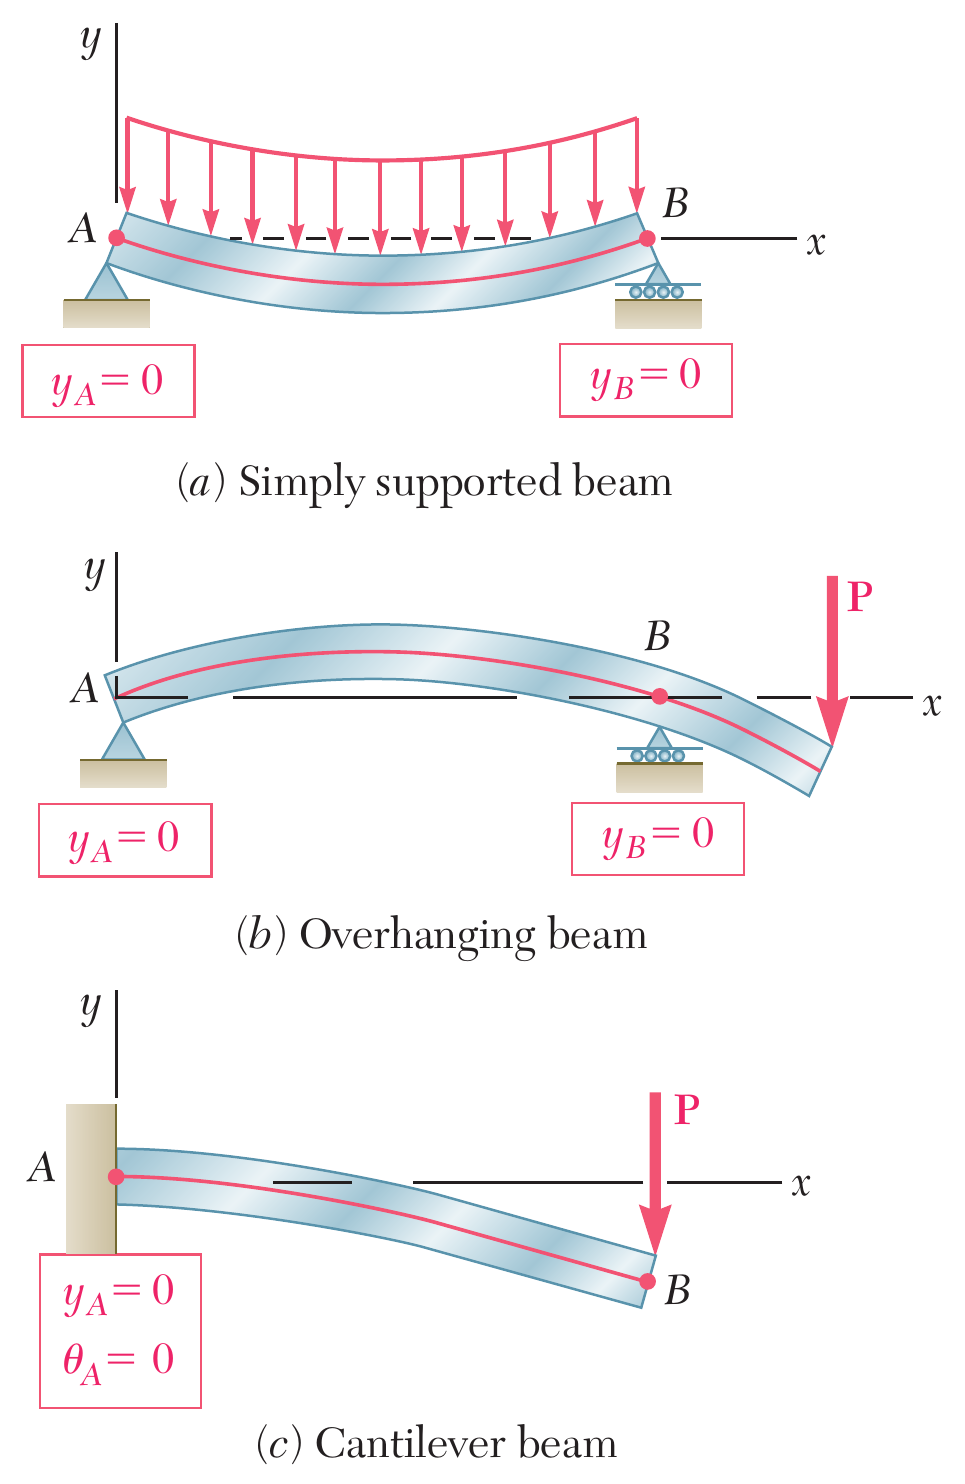
\includegraphics[width=\linewidth,height=1.9cm,keepaspectratio]{Chap_9/fig_9_8.png}
  \end{columns}
\end{frame}
% ===========
\section{Xác định trực tiếp đường đàn hồi từ tải trọng phân bố}
\begin{frame}[t]{Xác định trực tiếp đường đàn hồi từ tải trọng phân bố}
  \begin{columns}[T]
    \column{0.60\textwidth}
      \small
      \begin{itemize}
        \setlength{\itemsep}{0.5em}
        \item Với dầm chịu tải trọng phân bố:
        \[
          \frac{dM}{dx} = V(x) \qquad
          \frac{d^2M}{dx^2} = \frac{dV}{dx} = -w(x)
        \]
        \item Phương trình chuyển vị của dầm trở thành:
        \[
          \frac{d^2M}{dx^2} = EI\frac{d^4y}{dx^4} = -w(x)
        \]
        \item Tích phân bốn lần:
        \[
          EI\,y(x) = -\int dx\int dx\int dx\int w(x)\,dx
        \]
        \[
          \qquad + \tfrac{1}{6}C_1x^3 + \tfrac{1}{2}C_2x^2 + C_3x + C_4
        \]
        \item Các hằng số được xác định từ điều kiện biên.
      \end{itemize}
    \column{0.38\textwidth}
      \centering
      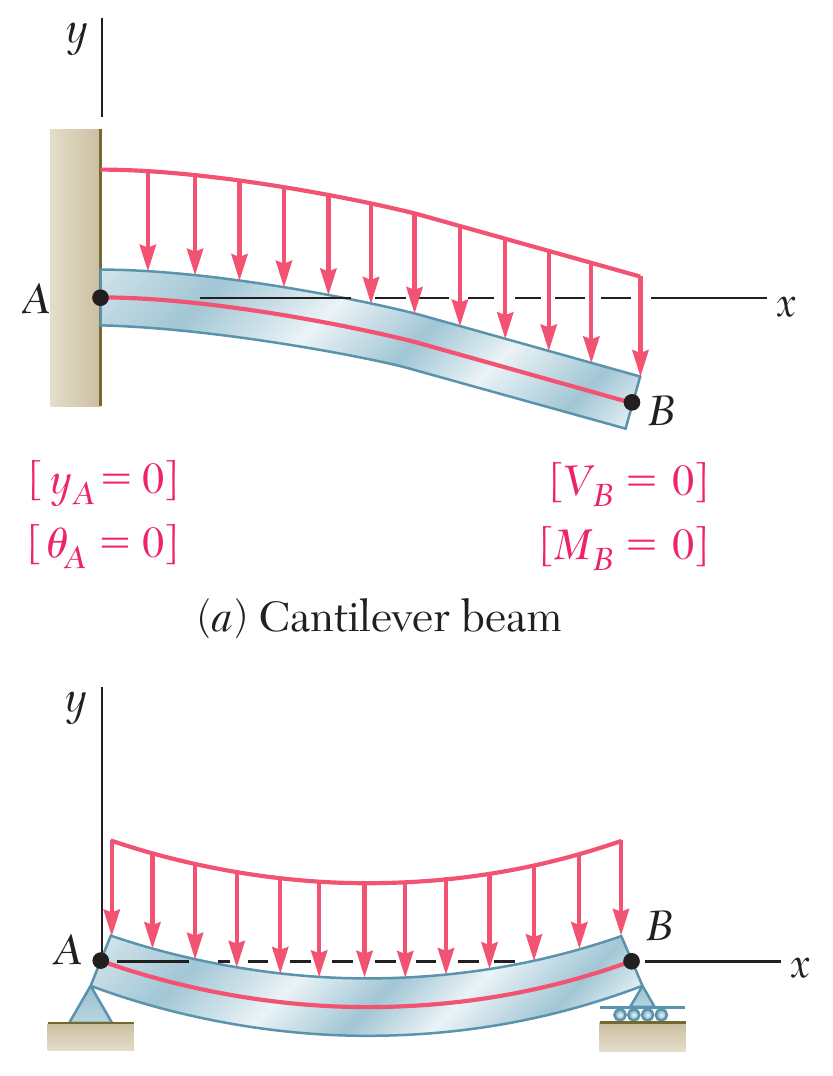
\includegraphics[width=\linewidth,height=2.9cm,keepaspectratio]{Chap_9/fig_9_20.png}\\[2pt]
      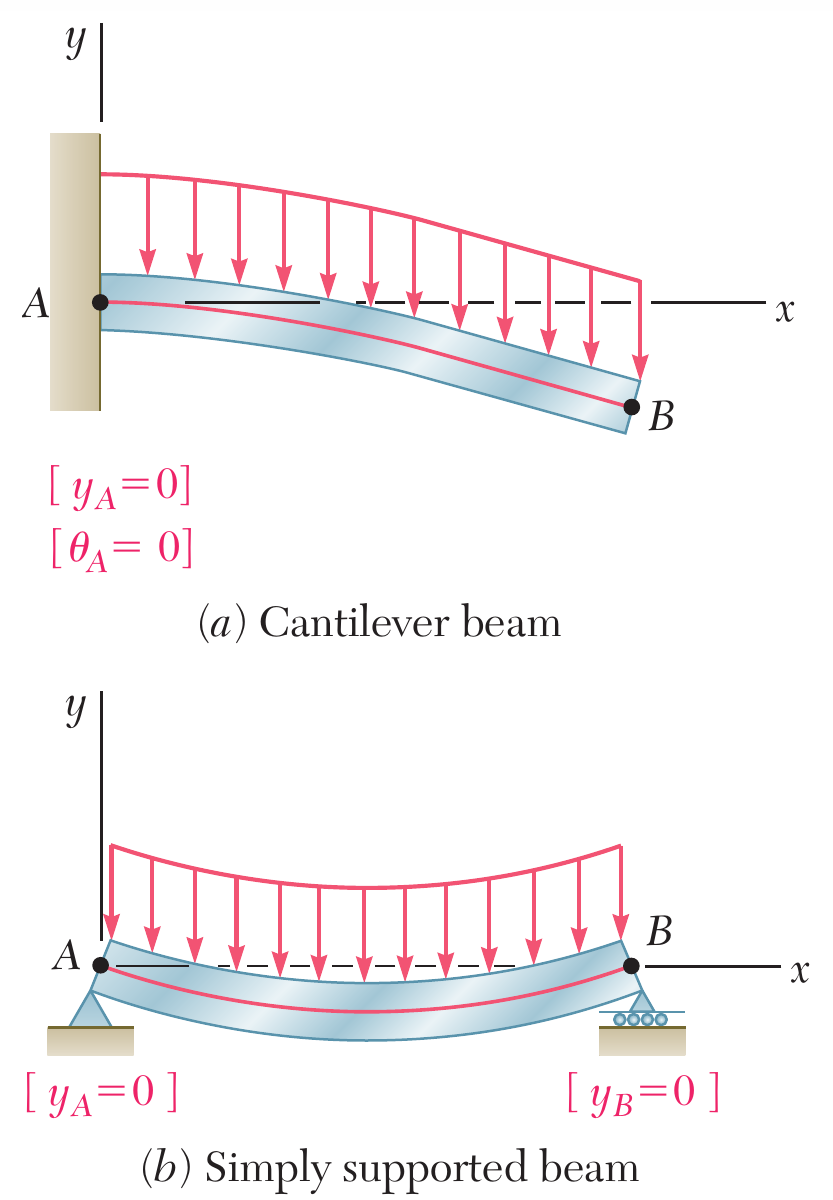
\includegraphics[width=\linewidth,height=2.9cm,keepaspectratio]{Chap_9/fig_9_1.png}
  \end{columns}
\end{frame}
% ===========
\section{Dầm siêu tĩnh}
\begin{frame}[t]{Dầm siêu tĩnh}
  \begin{columns}[T]
    \column{0.60\textwidth}
      \small
      \begin{itemize}
        \setlength{\itemsep}{0.4em}
        \item Xét dầm có ngàm tại $A$ và gối con lăn tại $B$.
        \item Từ sơ đồ vật thể tự do, có bốn thành phần phản lực chưa biết.
        \item Điều kiện cân bằng tĩnh học cho:
        \[
          \textstyle\sum F_x = 0 \qquad \sum F_y = 0 \qquad \sum M_A = 0
        \]
        Dầm là siêu tĩnh.
        \item Ngoài ra còn có phương trình độ võng của dầm:
        \[
          EI\,y = \int_0^x dx\int_0^x M(x)\,dx + C_1x + C_2
        \]
        phương trình này đưa vào hai ẩn số nhưng cho thêm ba phương trình từ
        các điều kiện biên:
        \[
          \text{Tại } x = 0:\ \theta = 0,\ y = 0 \qquad
          \text{Tại } x = L:\ y = 0
        \]
      \end{itemize}
    \column{0.38\textwidth}
      \centering
      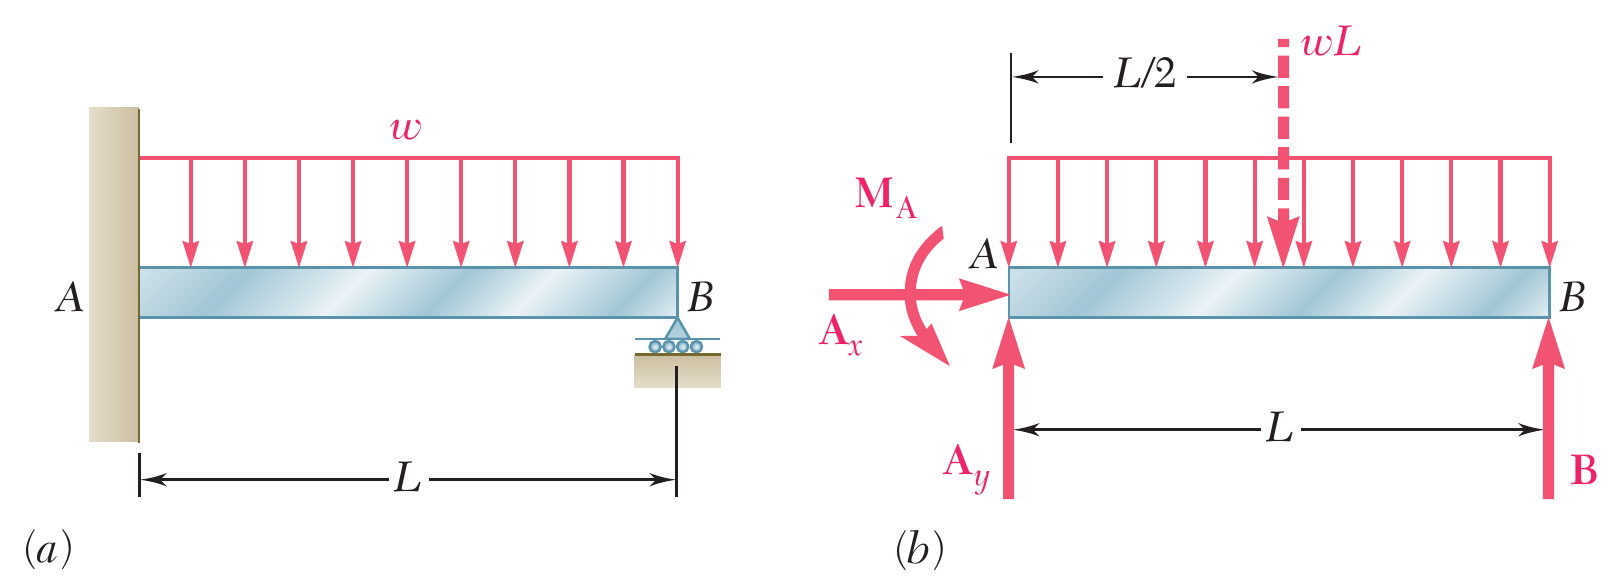
\includegraphics[width=\linewidth,height=1.9cm,keepaspectratio]{Chap_9/fig_9_23.png}\\[2pt]
      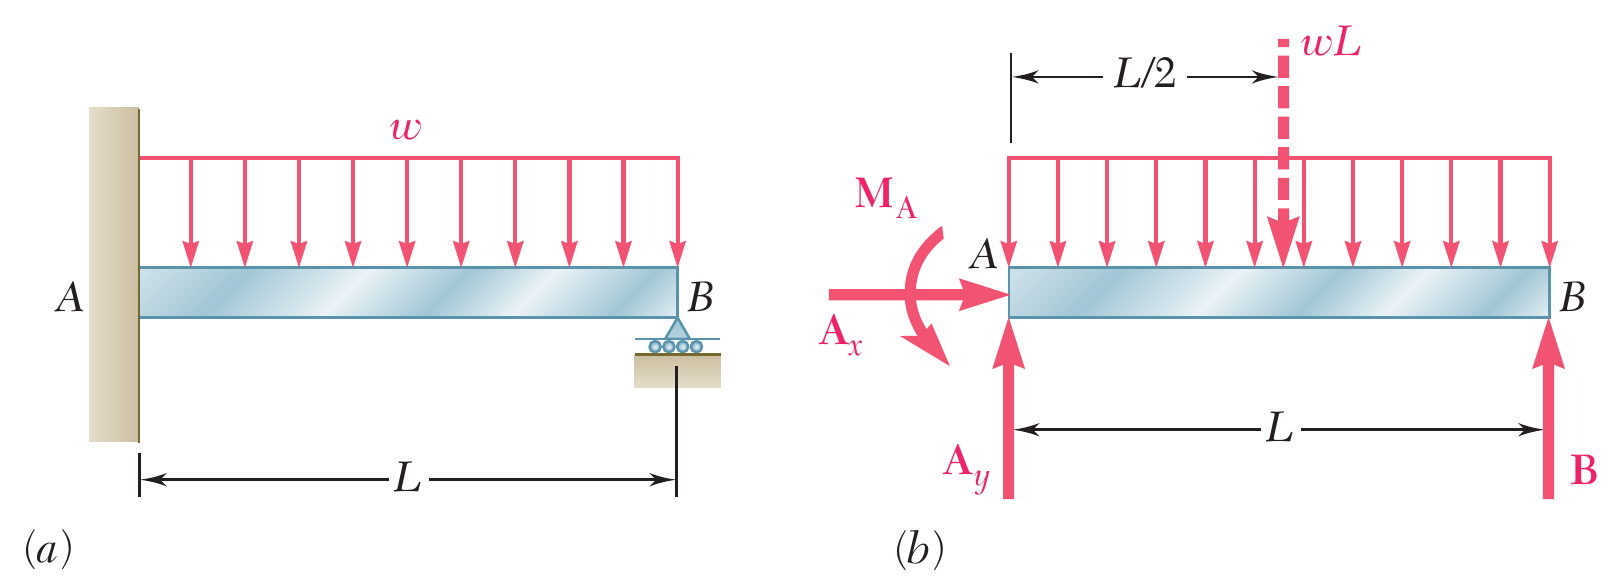
\includegraphics[width=\linewidth,height=1.9cm,keepaspectratio]{Chap_9/fig_9_23.png}\\[2pt]
      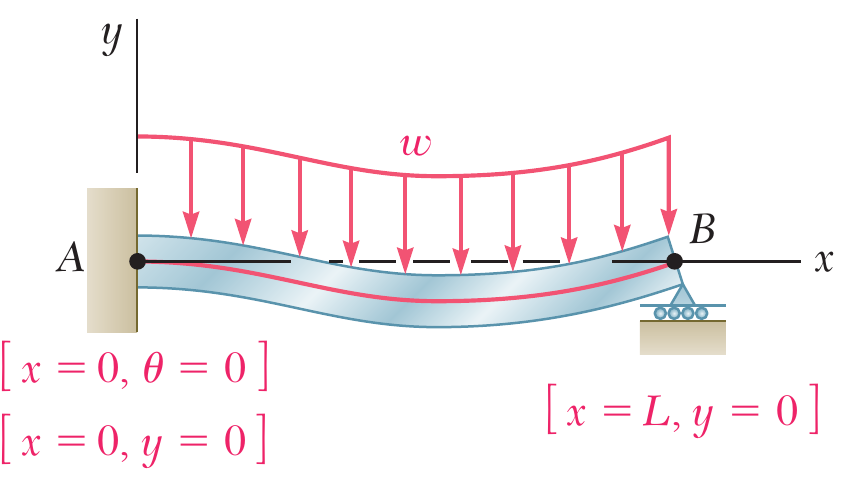
\includegraphics[width=\linewidth,height=1.9cm,keepaspectratio]{Chap_9/fig_9_24.png}
  \end{columns}
\end{frame}
% ===========
\section{Bài mẫu 9.1}
\begin{frame}[t]{Bài mẫu 9.1}
  \begin{columns}[T]
    \column{0.42\textwidth}
      \centering
      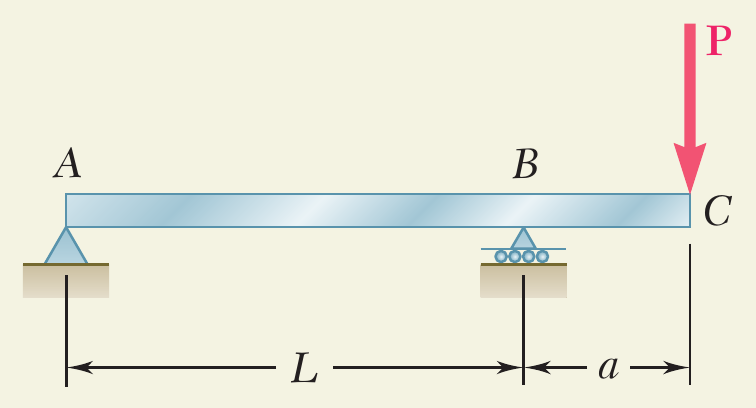
\includegraphics[width=\linewidth,height=5.5cm,keepaspectratio]{Chap_9/sp_9_1_a.png}
    \column{0.56\textwidth}
      \small
      Với đoạn $AB$ của dầm có đầu thừa, (a) thiết lập phương trình đường đàn
      hồi, (b) xác định độ võng lớn nhất, (c) tính $y_{\max}$ với các số liệu:
      W360$\times$101, $I = 300\times10^{6}\,\mathrm{mm}^4$,
      $E = 200\,\mathrm{GPa}$, $P = 200\,\mathrm{kN}$, $L = 4{,}5\,\mathrm{m}$,
      $a = 1{,}2\,\mathrm{m}$.

      \vspace{0.5em}
      \textbf{LỜI GIẢI:}
      \begin{itemize}
        \setlength{\itemsep}{0.3em}
        \item Thiết lập biểu thức $M(x)$ và phương trình vi phân của đường đàn
              hồi.
        \item Tích phân phương trình vi phân hai lần và áp dụng điều kiện biên
              để nhận được đường đàn hồi.
        \item Xác định điểm có góc xoay bằng không, hay điểm có độ võng lớn
              nhất.
        \item Tính độ võng lớn nhất tương ứng.
      \end{itemize}
  \end{columns}
\end{frame}
% ===========
\begin{frame}[t]{Bài mẫu 9.1 (tiếp)}
  \begin{columns}[T]
    \column{0.56\textwidth}
      \small
      \textbf{LỜI GIẢI:}
      \begin{itemize}
        \setlength{\itemsep}{0.5em}
        \item Thiết lập biểu thức $M(x)$ và phương trình vi phân của đường đàn
              hồi.

              Phản lực:
        \[
          R_A = \frac{Pa}{L}\downarrow \qquad
          R_B = P\left(1 + \frac{a}{L}\right)\uparrow
        \]
              Từ sơ đồ vật thể tự do của đoạn $AD$:
        \[
          M = -P\frac{a}{L}x \qquad (0 < x < L)
        \]
              Phương trình vi phân của đường đàn hồi:
        \[
          EI\frac{d^2y}{dx^2} = -P\frac{a}{L}x
        \]
      \end{itemize}
    \column{0.42\textwidth}
      \centering
      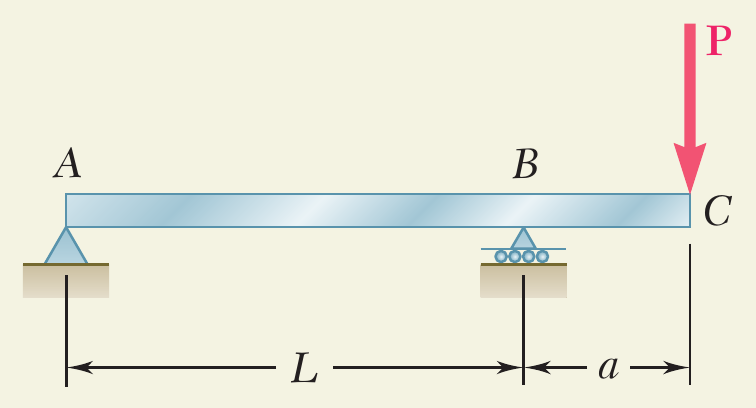
\includegraphics[width=\linewidth,height=1.9cm,keepaspectratio]{Chap_9/sp_9_1_a.png}\\[2pt]
      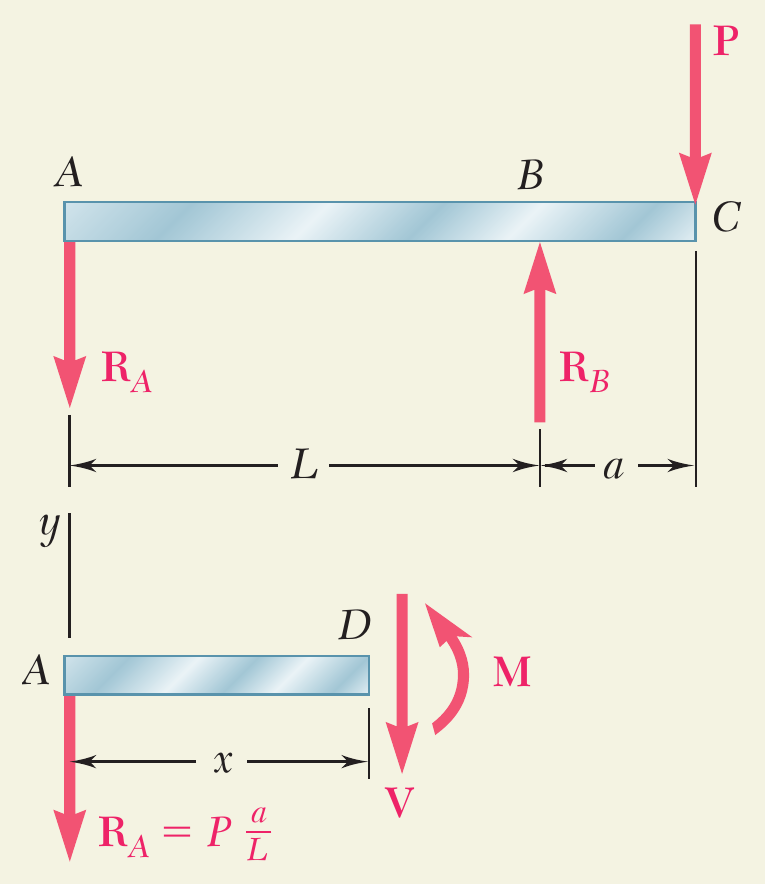
\includegraphics[width=\linewidth,height=1.9cm,keepaspectratio]{Chap_9/sp_9_1_b.png}\\[2pt]
      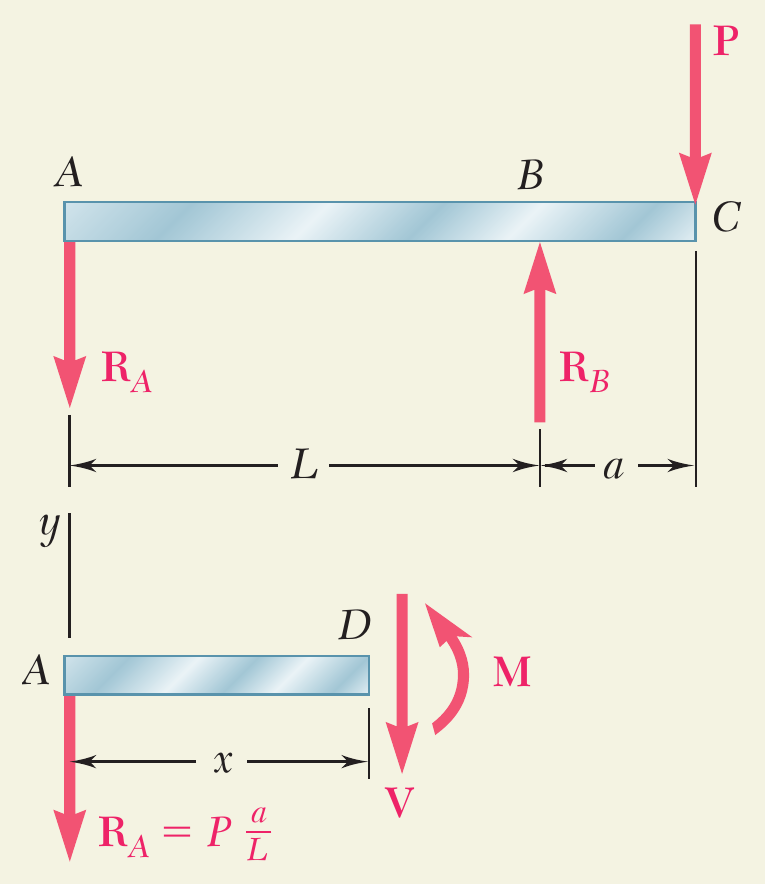
\includegraphics[width=\linewidth,height=1.9cm,keepaspectratio]{Chap_9/sp_9_1_b.png}
  \end{columns}
\end{frame}
% ===========
\begin{frame}[t]{Bài mẫu 9.1 (tiếp)}
  \begin{columns}[T]
    \column{0.70\textwidth}
      \footnotesize
      \begin{itemize}
        \setlength{\itemsep}{0.3em}
        \item Tích phân phương trình vi phân hai lần và áp dụng điều kiện biên
              để nhận được đường đàn hồi:
        \[
          EI\frac{dy}{dx} = -\frac{1}{2}P\frac{a}{L}x^2 + C_1
          \qquad
          EI\,y = -\frac{1}{6}P\frac{a}{L}x^3 + C_1x + C_2
        \]
        \[
          \begin{aligned}
            &\text{tại } x = 0,\ y = 0: && C_2 = 0\\
            &\text{tại } x = L,\ y = 0: && 0 = -\tfrac{1}{6}P\tfrac{a}{L}L^3 + C_1L
              \quad\Rightarrow\quad C_1 = \tfrac{1}{6}PaL
          \end{aligned}
        \]
        \item Thay vào:
        \[
          EI\frac{dy}{dx} = -\frac{1}{2}P\frac{a}{L}x^2 + \frac{1}{6}PaL
          \qquad
          \frac{dy}{dx} = \frac{PaL}{6EI}\left[1 - 3\left(\frac{x}{L}\right)^2\right]
        \]
        \[
          EI\,y = -\frac{1}{6}P\frac{a}{L}x^3 + \frac{1}{6}PaLx
          \qquad
          \boxed{y = \frac{PaL^2}{6EI}\left[\frac{x}{L} - \left(\frac{x}{L}\right)^3\right]}
        \]
      \end{itemize}
    \column{0.28\textwidth}
      \centering
      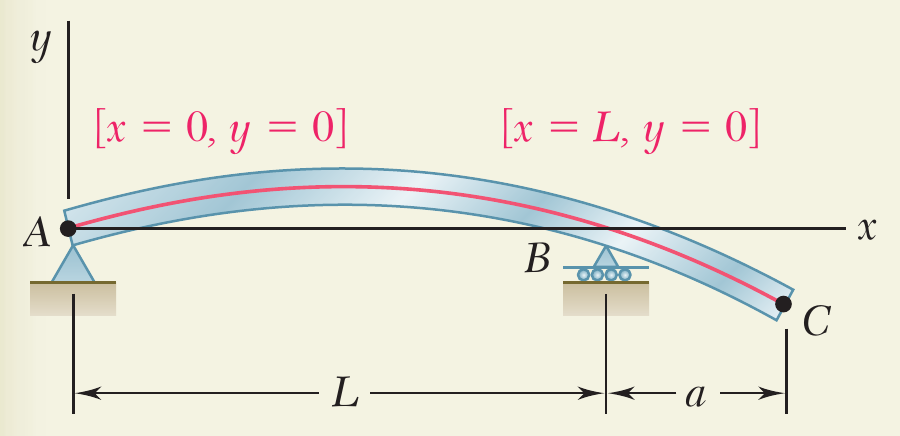
\includegraphics[width=\linewidth,height=4.5cm,keepaspectratio]{Chap_9/sp_9_1_c.png}
  \end{columns}
\end{frame}
% ===========
\begin{frame}[t]{Bài mẫu 9.1 (tiếp)}
  \begin{columns}[T]
    \column{0.60\textwidth}
      \small
      \begin{itemize}
        \setlength{\itemsep}{0.5em}
        \item Xác định điểm có góc xoay bằng không, hay điểm có độ võng lớn
              nhất:
        \[
          \frac{dy}{dx} = 0 = \frac{PaL}{6EI}\left[1 - 3\left(\frac{x_m}{L}\right)^2\right]
          \qquad x_m = \frac{L}{\sqrt{3}} = 0{,}577L
        \]
        \item Tính độ võng lớn nhất tương ứng:
        \[
          y_{\max} = \frac{PaL^2}{6EI}\left[0{,}577 - (0{,}577)^3\right]
          \qquad y_{\max} = 0{,}0642\frac{PaL^2}{EI}
        \]
        \[
          y_{\max} = 0{,}0642\frac{(200\times10^{3}\,\mathrm{N})(1{,}2\,\mathrm{m})(4{,}5\,\mathrm{m})^2}
                                  {(200\times10^{9}\,\mathrm{Pa})(300\times10^{-6}\,\mathrm{m}^4)}
        \]
        \[
          \boxed{y_{\max} = 5{,}2\,\mathrm{mm}}
        \]
      \end{itemize}
    \column{0.38\textwidth}
      \centering
      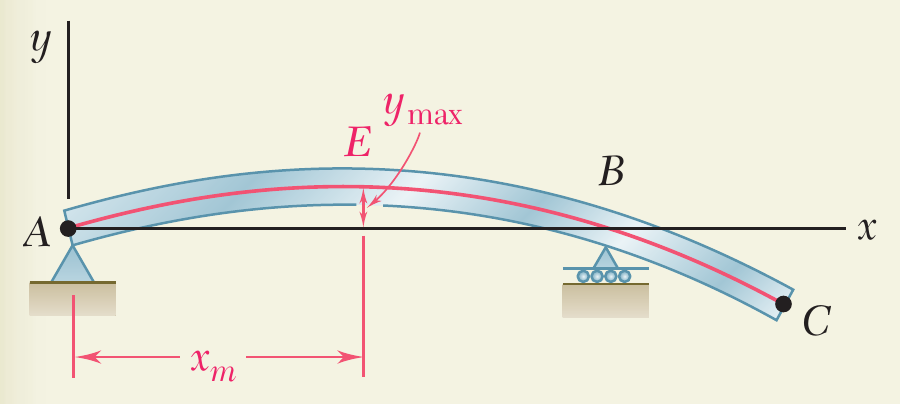
\includegraphics[width=\linewidth,height=5.5cm,keepaspectratio]{Chap_9/sp_9_1_d.png}
  \end{columns}
\end{frame}
% ===========
\section{Bài mẫu 9.3}
\begin{frame}[t]{Bài mẫu 9.3}
  \begin{columns}[T]
    \column{0.42\textwidth}
      \centering
      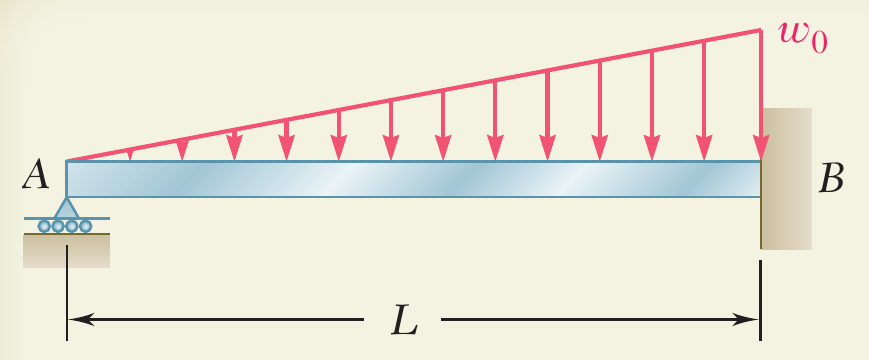
\includegraphics[width=\linewidth,height=5.5cm,keepaspectratio]{Chap_9/sp_9_3_a.png}
    \column{0.56\textwidth}
      \small
      Với dầm đồng chất như hình vẽ, xác định phản lực tại $A$, thiết lập
      phương trình đường đàn hồi và xác định góc xoay tại $A$. (Lưu ý rằng dầm
      là siêu tĩnh bậc một.)

      \vspace{0.8em}
      \textbf{LỜI GIẢI:}
      \begin{itemize}
        \setlength{\itemsep}{0.5em}
        \item Thiết lập phương trình vi phân của đường đàn hồi (phụ thuộc vào
              phản lực tại $A$).
        \item Tích phân hai lần và áp dụng điều kiện biên để tìm phản lực tại
              $A$ và nhận được đường đàn hồi.
        \item Tính góc xoay tại $A$.
      \end{itemize}
  \end{columns}
\end{frame}
% ===========
\begin{frame}[t]{Bài mẫu 9.3 (tiếp)}
  \begin{columns}[T]
    \column{0.56\textwidth}
      \small
      \begin{itemize}
        \setlength{\itemsep}{0.6em}
        \item Xét mô men tác dụng tại mặt cắt $D$:
        \[
          \textstyle\sum M_D = 0:\quad
          R_Ax - \frac{1}{2}\left(\frac{w_0x^2}{L}\right)\frac{x}{3} - M = 0
        \]
        \[
          M = R_Ax - \frac{w_0x^3}{6L}
        \]
        \item Phương trình vi phân của đường đàn hồi:
        \[
          EI\frac{d^2y}{dx^2} = M = R_Ax - \frac{w_0x^3}{6L}
        \]
      \end{itemize}
    \column{0.42\textwidth}
      \centering
      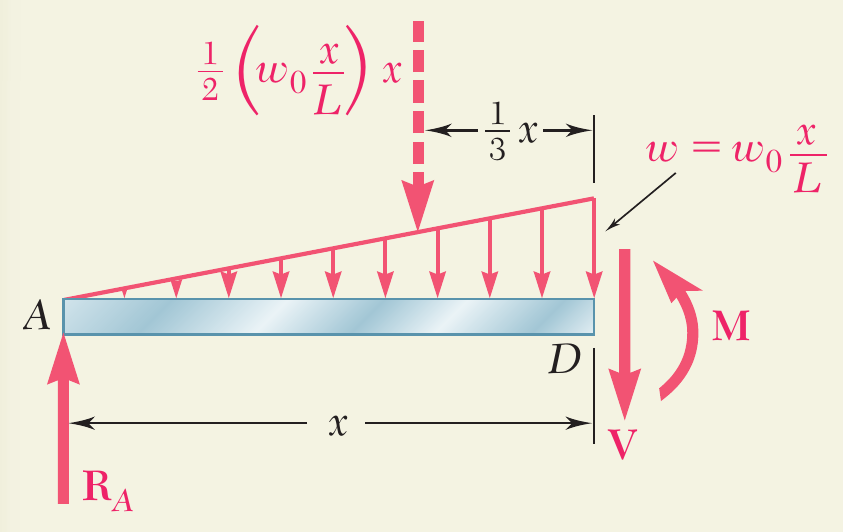
\includegraphics[width=\linewidth,height=5.5cm,keepaspectratio]{Chap_9/sp_9_3_b.png}
  \end{columns}
\end{frame}
% ===========
\begin{frame}[t]{Bài mẫu 9.3 (tiếp)}
  \begin{columns}[T]
    \column{0.62\textwidth}
      \footnotesize
      \begin{itemize}
        \setlength{\itemsep}{0.3em}
        \item Tích phân hai lần:
        \[
          EI\frac{dy}{dx} = EI\theta = \tfrac{1}{2}R_Ax^2 - \frac{w_0x^4}{24L} + C_1
        \]
        \[
          EI\,y = \tfrac{1}{6}R_Ax^3 - \frac{w_0x^5}{120L} + C_1x + C_2
        \]
        \item Áp dụng điều kiện biên:
        \[
          \text{tại } x = 0,\ y = 0:\quad C_2 = 0
        \]
        \[
          \text{tại } x = L,\ \theta = 0:\quad
          \tfrac{1}{2}R_AL^2 - \frac{w_0L^3}{24} + C_1 = 0
        \]
        \[
          \text{tại } x = L,\ y = 0:\quad
          \tfrac{1}{6}R_AL^3 - \frac{w_0L^4}{120} + C_1L + C_2 = 0
        \]
        \item Giải ra phản lực tại $A$:
        \[
          \tfrac{1}{3}R_AL^3 - \tfrac{1}{30}w_0L^4 = 0
          \qquad \boxed{R_A = \tfrac{1}{10}w_0L\uparrow}
        \]
      \end{itemize}
    \column{0.36\textwidth}
      \centering
      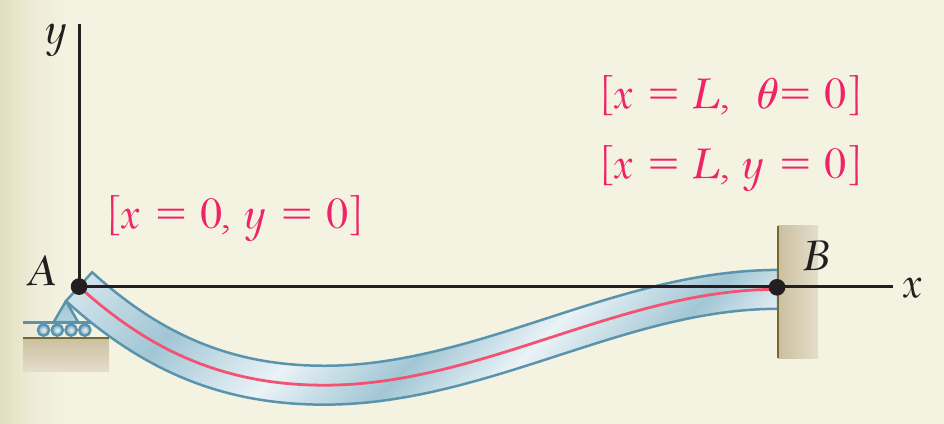
\includegraphics[width=\linewidth,height=5.5cm,keepaspectratio]{Chap_9/sp_9_3_c.png}
  \end{columns}
\end{frame}
% ===========
\begin{frame}[t]{Bài mẫu 9.3 (tiếp)}
  \begin{columns}[T]
    \column{0.60\textwidth}
      \small
      \begin{itemize}
        \setlength{\itemsep}{0.5em}
        \item Thay $C_1$, $C_2$ và $R_A$ vào phương trình đường đàn hồi:
        \[
          EI\,y = \tfrac{1}{6}\left(\tfrac{1}{10}w_0L\right)x^3
            - \frac{w_0x^5}{120L} - \left(\tfrac{1}{120}w_0L^3\right)x
        \]
        \[
          \boxed{y = \frac{w_0}{120EIL}\left(-x^5 + 2L^2x^3 - L^4x\right)}
        \]
        \item Đạo hàm một lần để tìm góc xoay:
        \[
          \theta = \frac{dy}{dx} = \frac{w_0}{120EIL}\left(-5x^4 + 6L^2x^2 - L^4\right)
        \]
        tại $x = 0$:
        \[
          \boxed{\theta_A = -\frac{w_0L^3}{120EI}}
        \]
      \end{itemize}
    \column{0.38\textwidth}
      \centering
      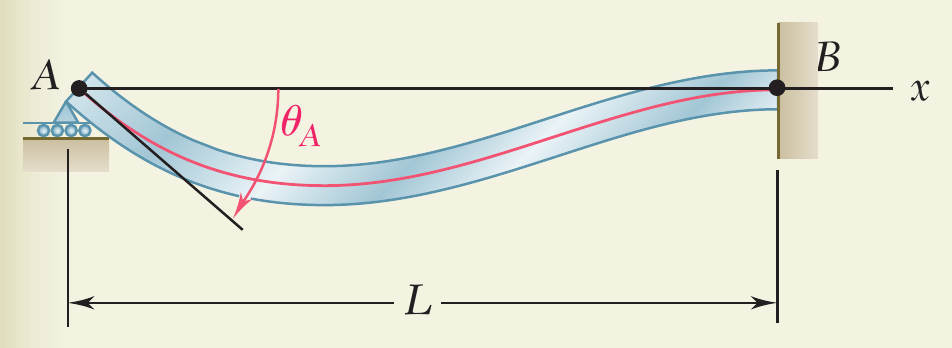
\includegraphics[width=\linewidth,height=5.5cm,keepaspectratio]{Chap_9/sp_9_3_d.png}
  \end{columns}
\end{frame}
% ===========
\section{Phương pháp cộng tác dụng}
\begin{frame}[t]{Phương pháp cộng tác dụng}
  \begin{columns}[T]
    \column{0.50\textwidth}
      \small
      \textbf{Nguyên lý cộng tác dụng:}
      \begin{itemize}
        \setlength{\itemsep}{0.8em}
        \item Biến dạng của dầm chịu tổ hợp tải trọng có thể nhận được bằng
              tổ hợp tuyến tính các biến dạng do từng tải trọng riêng rẽ.
        \item Quá trình tính toán được thuận tiện hơn nhờ các bảng lời giải cho
              các dạng tải trọng và liên kết thông dụng.
      \end{itemize}
    \column{0.48\textwidth}
      \centering
      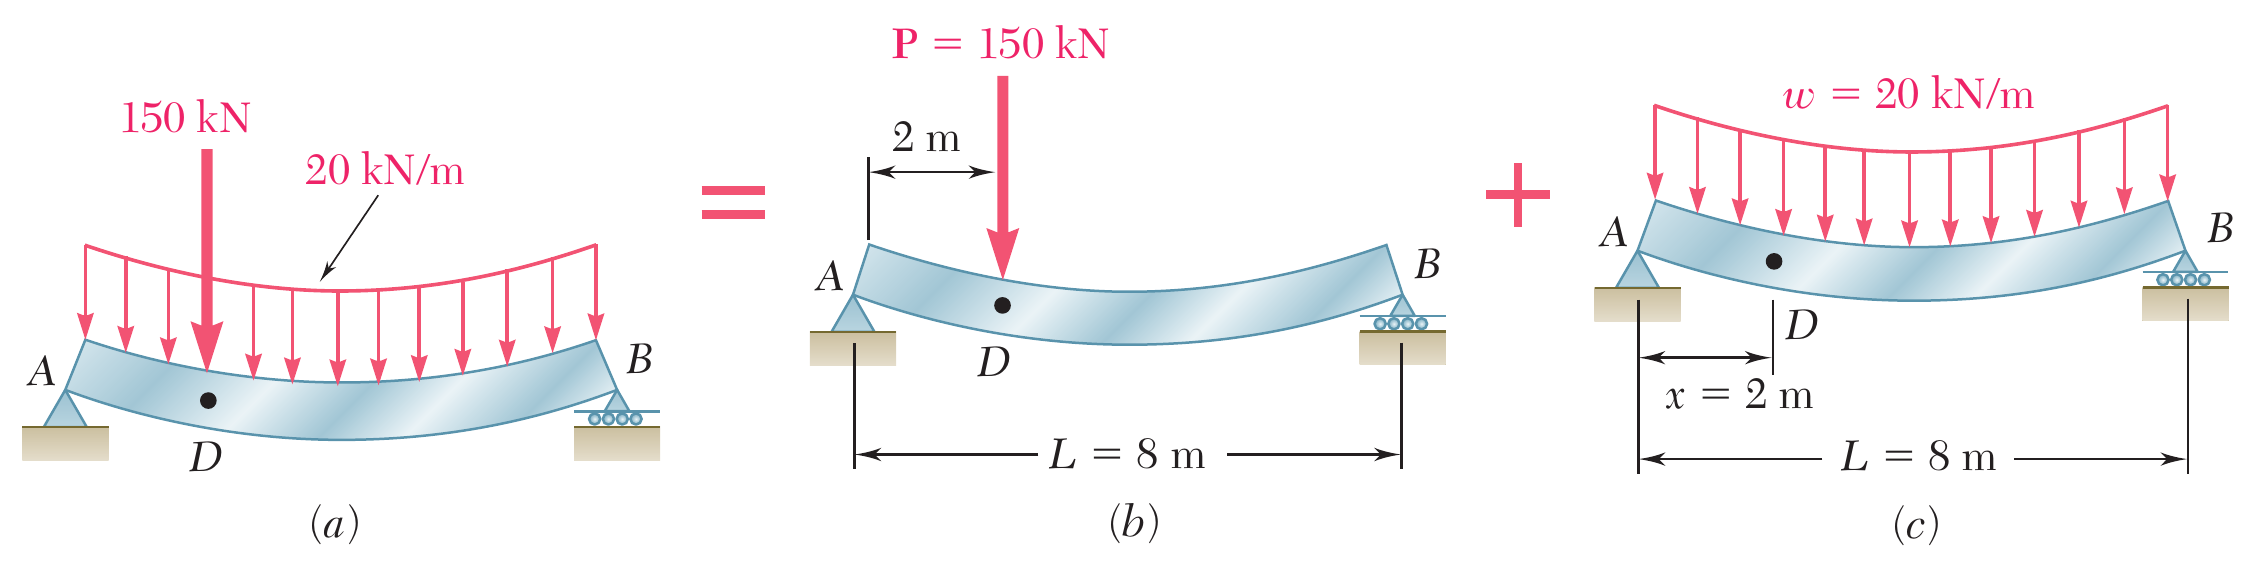
\includegraphics[width=\linewidth,height=6cm,keepaspectratio]{Chap_9/fig_9_32.png}
  \end{columns}
\end{frame}
% ===========
\section{Bài mẫu 9.7}
\begin{frame}[t]{Bài mẫu 9.7}
  \begin{columns}[T]
    \column{0.40\textwidth}
      \small
      Với dầm và tải trọng như hình vẽ, xác định góc xoay và độ võng tại
      điểm $B$.

      \vspace{0.8em}
      \textbf{LỜI GIẢI:}

      Cộng tác dụng các biến dạng do Tải trọng I và Tải trọng II như hình vẽ.
    \column{0.58\textwidth}
      \centering
      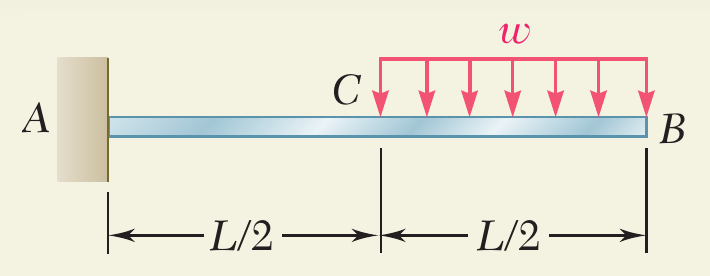
\includegraphics[width=\linewidth,height=2.9cm,keepaspectratio]{Chap_9/sp_9_7_a.png}\\[2pt]
      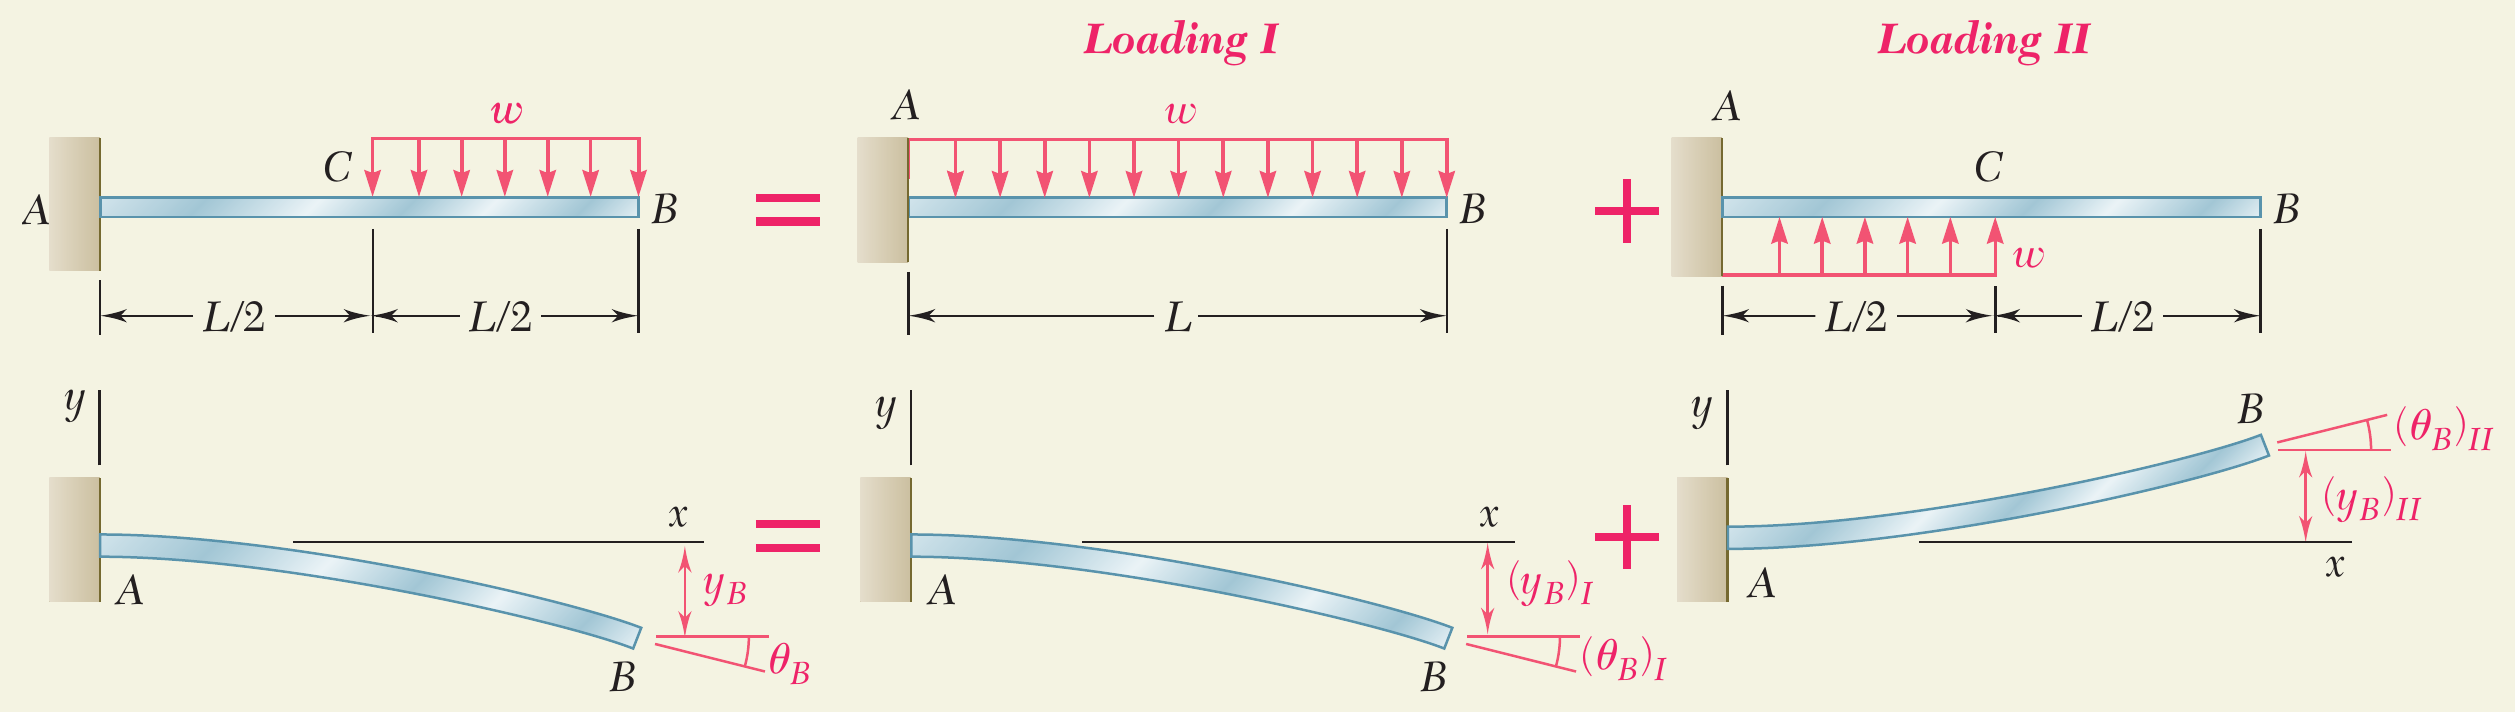
\includegraphics[width=\linewidth,height=2.9cm,keepaspectratio]{Chap_9/sp_9_7_b.png}
  \end{columns}
\end{frame}
% ===========
\begin{frame}[t]{Bài mẫu 9.7 (tiếp)}
  \begin{columns}[T]
    \column{0.49\textwidth}
      \small
      \textbf{Tải trọng I}
      \[
        (\theta_B)_I = -\frac{wL^3}{6EI}
        \qquad
        (y_B)_I = -\frac{wL^4}{8EI}
      \]
      \centering
      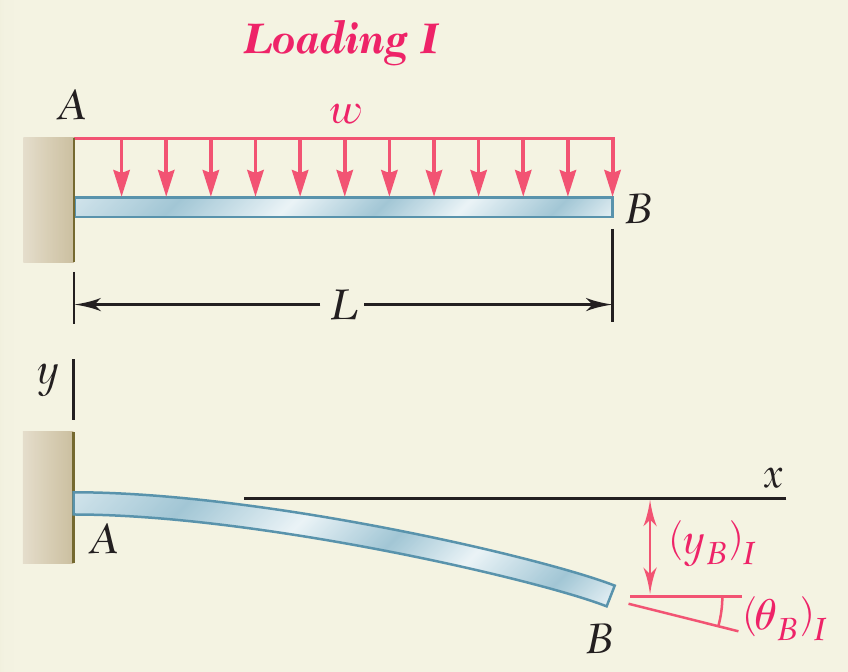
\includegraphics[width=\linewidth,height=2.6cm,keepaspectratio]{Chap_9/sp_9_7_c.png}
    \column{0.49\textwidth}
      \small
      \textbf{Tải trọng II}
      \[
        (\theta_C)_{II} = \frac{wL^3}{48EI}
        \qquad
        (y_C)_{II} = \frac{wL^4}{128EI}
      \]
      Trên đoạn dầm $CB$, mô men uốn bằng không và đường đàn hồi là đường
      thẳng:
      \[
        (\theta_B)_{II} = (\theta_C)_{II} = \frac{wL^3}{48EI}
      \]
      \[
        (y_B)_{II} = \frac{wL^4}{128EI} + \frac{wL^3}{48EI}\left(\frac{L}{2}\right)
          = \frac{7wL^4}{384EI}
      \]
      \centering
      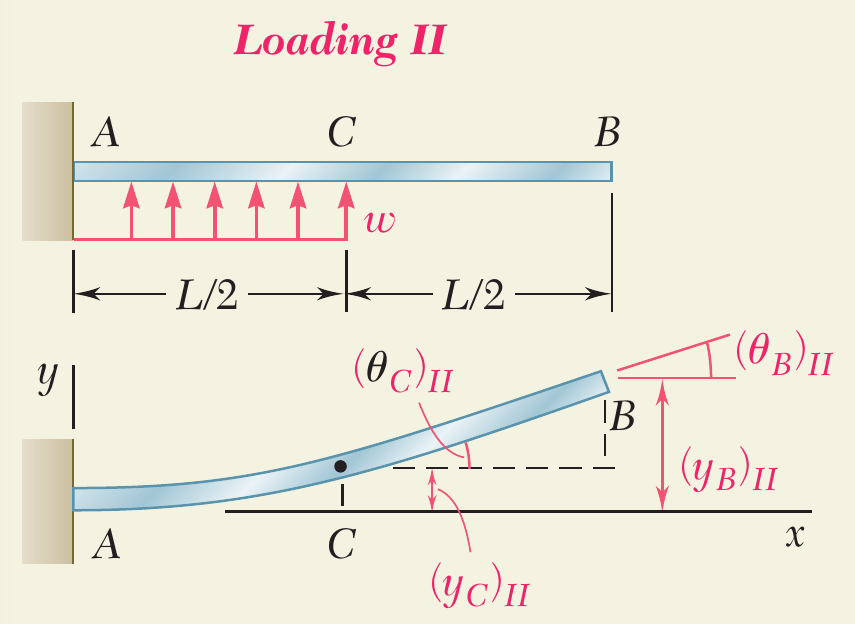
\includegraphics[width=\linewidth,height=1.8cm,keepaspectratio]{Chap_9/sp_9_7_d.png}
  \end{columns}
\end{frame}
% ===========
\begin{frame}[t]{Bài mẫu 9.7 (tiếp)}
  \begin{columns}[T]
    \column{0.56\textwidth}
      \small
      Kết hợp hai lời giải:
      \[
        \theta_B = (\theta_B)_I + (\theta_B)_{II}
          = -\frac{wL^3}{6EI} + \frac{wL^3}{48EI}
        \qquad \boxed{\theta_B = -\frac{7wL^3}{48EI}}
      \]
      \[
        y_B = (y_B)_I + (y_B)_{II}
          = -\frac{wL^4}{8EI} + \frac{7wL^4}{384EI}
        \qquad \boxed{y_B = -\frac{41wL^4}{384EI}}
      \]
    \column{0.42\textwidth}
      \centering
      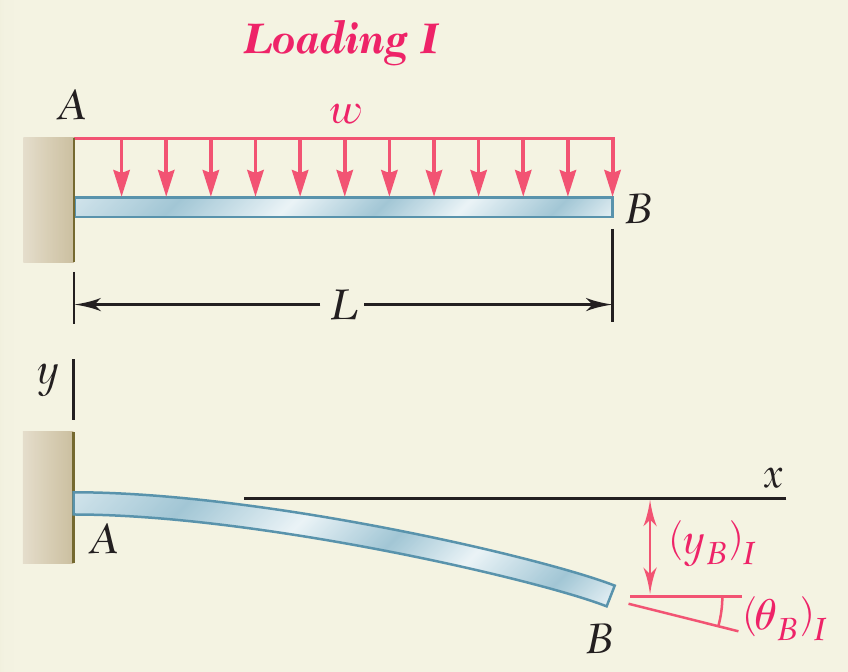
\includegraphics[width=\linewidth,height=5.5cm,keepaspectratio]{Chap_9/sp_9_7_c.png}
  \end{columns}
\end{frame}
% ===========
\section{Áp dụng cộng tác dụng cho dầm siêu tĩnh}
\begin{frame}[t]{Áp dụng phương pháp cộng tác dụng cho dầm siêu tĩnh}
  \begin{columns}[T]
    \column{0.58\textwidth}
      \small
      \begin{itemize}
        \setlength{\itemsep}{0.7em}
        \item Phương pháp cộng tác dụng có thể được áp dụng để xác định phản
              lực tại các gối của dầm siêu tĩnh.
        \item Chọn một phản lực làm phản lực thừa và loại bỏ hoặc thay đổi gối
              tương ứng.
        \item Xác định biến dạng của dầm khi không có gối thừa.
        \item Coi phản lực thừa là một tải trọng chưa biết, cùng với các tải
              trọng khác, phải tạo ra các biến dạng tương thích với các gối ban
              đầu.
      \end{itemize}
    \column{0.40\textwidth}
      \centering
      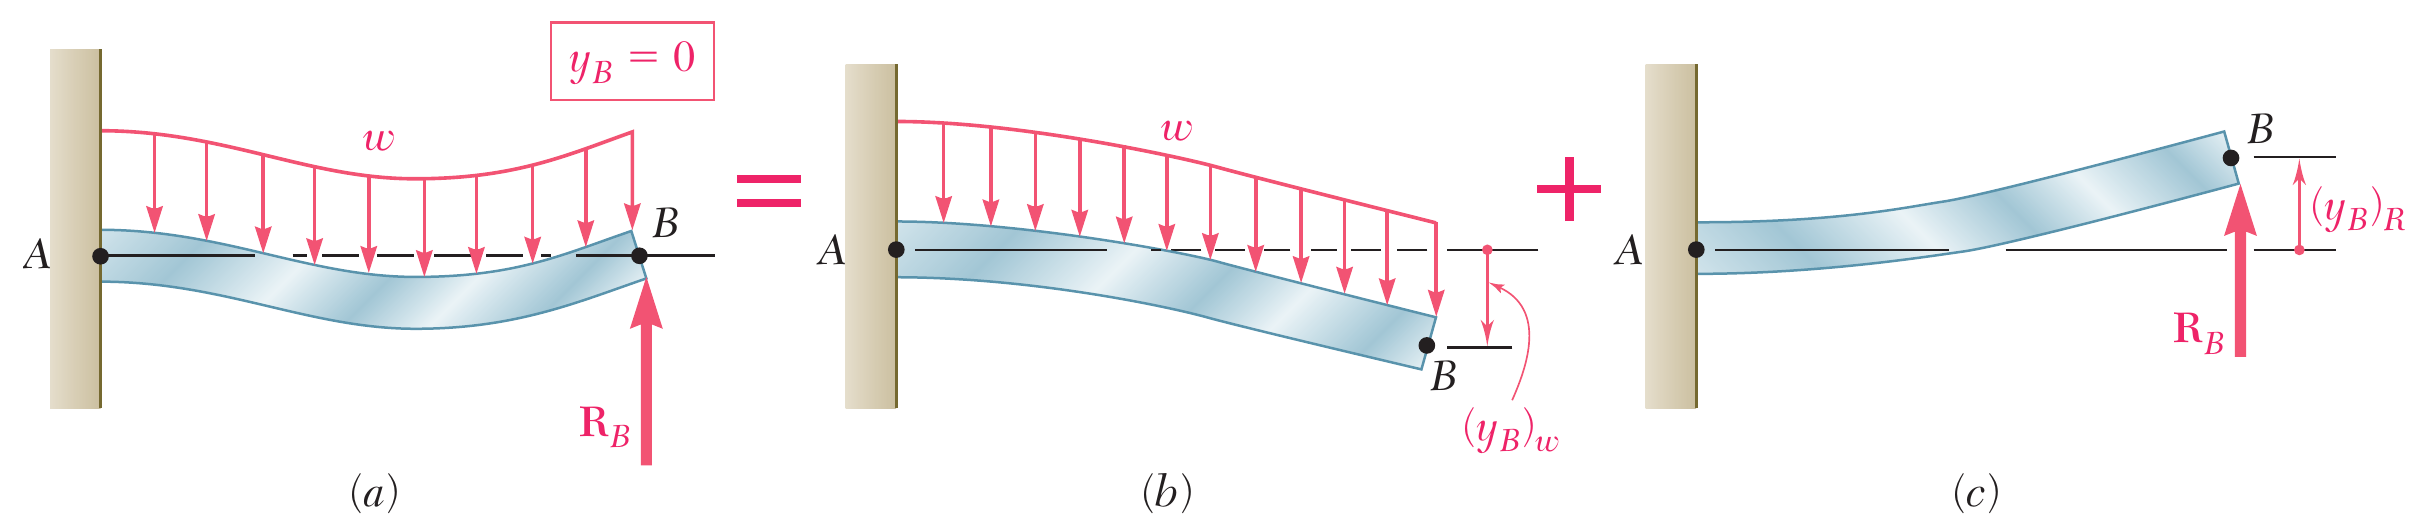
\includegraphics[width=\linewidth,height=5.5cm,keepaspectratio]{Chap_9/fig_9_34.png}
  \end{columns}
\end{frame}
% ===========
\section{Bài mẫu 9.8}
\begin{frame}[t]{Bài mẫu 9.8}
  \begin{columns}[T]
    \column{0.42\textwidth}
      \small
      Với dầm đồng chất và tải trọng như hình vẽ, xác định phản lực tại mỗi
      gối và góc xoay tại đầu $A$.

      \vspace{0.8em}
      \textbf{LỜI GIẢI:}
      \begin{itemize}
        \setlength{\itemsep}{0.5em}
        \item Giải phóng gối ``thừa'' tại $B$ và tìm biến dạng.
        \item Đặt phản lực tại $B$ như một tải trọng chưa biết để buộc chuyển
              vị tại $B$ bằng không.
      \end{itemize}
    \column{0.56\textwidth}
      \centering
      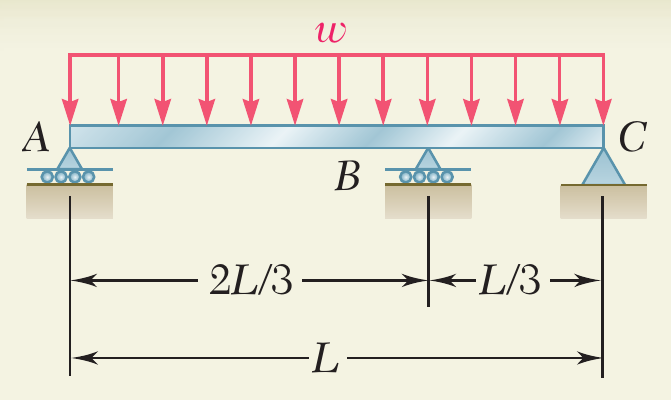
\includegraphics[width=\linewidth,height=2.9cm,keepaspectratio]{Chap_9/sp_9_8_a.png}\\[2pt]
      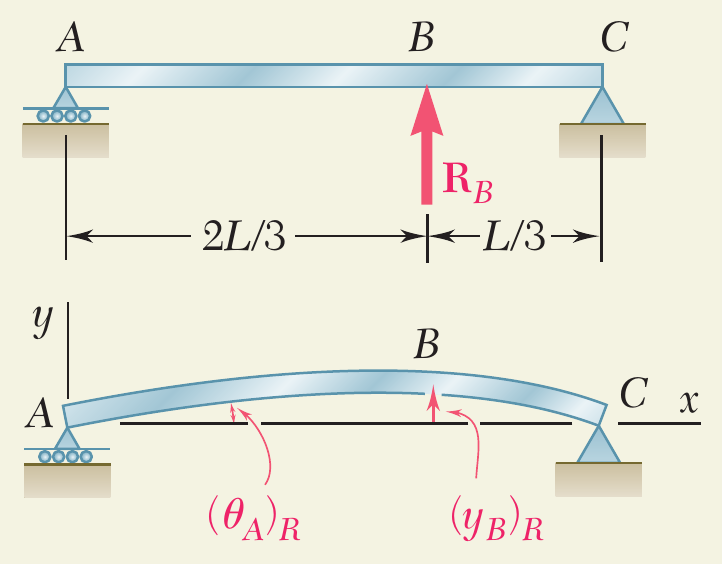
\includegraphics[width=\linewidth,height=2.9cm,keepaspectratio]{Chap_9/sp_9_8_c.png}
  \end{columns}
\end{frame}
% ===========
\begin{frame}[t]{Bài mẫu 9.8 (tiếp)}
  \begin{columns}[T]
    \column{0.56\textwidth}
      \small
      \begin{itemize}
        \item Tải trọng phân bố:
      \end{itemize}
      \[
        (y_B)_w = -\frac{w}{24EI}\left[x^4 - 2Lx^3 + L^3x\right]
      \]
      Tại điểm $B$, $x = \tfrac{2}{3}L$:
      \[
        (y_B)_w = -\frac{w}{24EI}\left[\left(\tfrac{2}{3}L\right)^4
          - 2L\left(\tfrac{2}{3}L\right)^3 + L^3\left(\tfrac{2}{3}L\right)\right]
      \]
      \[
        (y_B)_w = -0{,}01132\frac{wL^4}{EI}
      \]
    \column{0.42\textwidth}
      \centering
      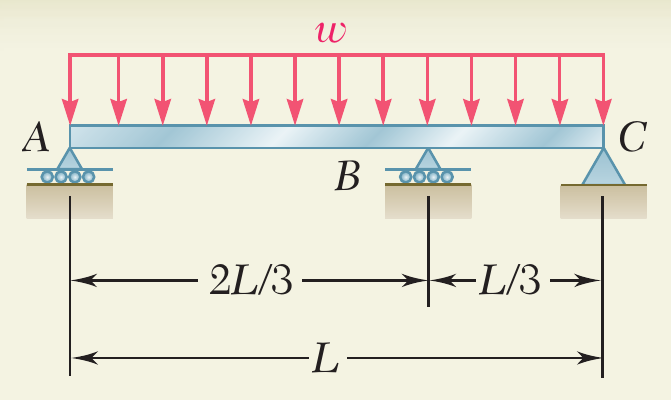
\includegraphics[width=\linewidth,height=2.9cm,keepaspectratio]{Chap_9/sp_9_8_a.png}\\[2pt]
      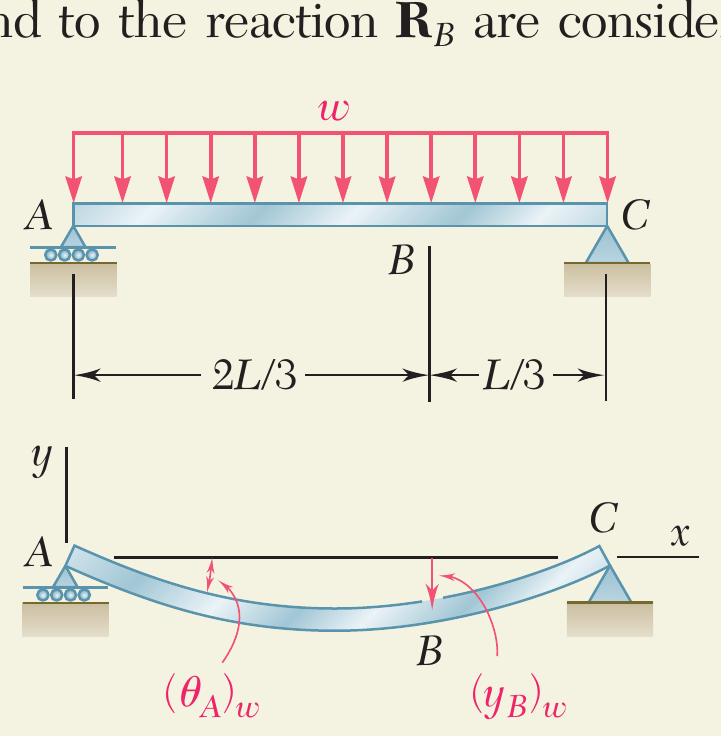
\includegraphics[width=\linewidth,height=2.9cm,keepaspectratio]{Chap_9/sp_9_8_b.png}
  \end{columns}
\end{frame}
% ===========
\begin{frame}[t]{Bài mẫu 9.8 (tiếp)}
  \begin{columns}[T]
    \column{0.56\textwidth}
      \small
      \begin{itemize}
        \item Tải trọng do phản lực thừa:
      \end{itemize}
      Tại $x = a$:
      \[
        y = -\frac{Pa^2b^2}{3EIL}
      \]
      Với $a = \tfrac{2}{3}L$ và $b = \tfrac{1}{3}L$:
      \[
        (y_B)_R = \frac{R_B}{3EIL}\left(\tfrac{2}{3}L\right)^2\left(\tfrac{L}{3}\right)^2
          = 0{,}01646\frac{R_BL^3}{EI}
      \]
    \column{0.42\textwidth}
      \centering
      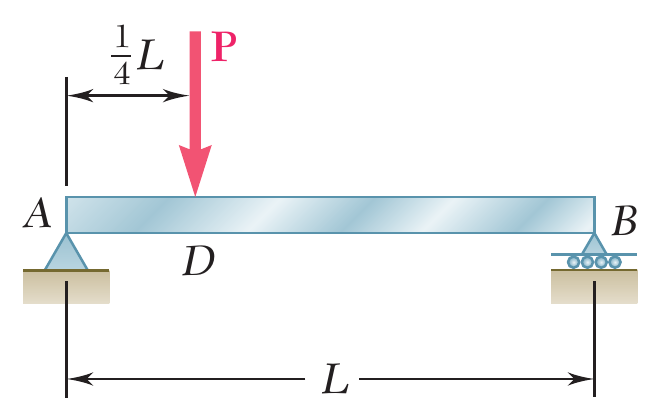
\includegraphics[width=\linewidth,height=2.9cm,keepaspectratio]{Chap_9/fig_9_60.png}\\[2pt]
      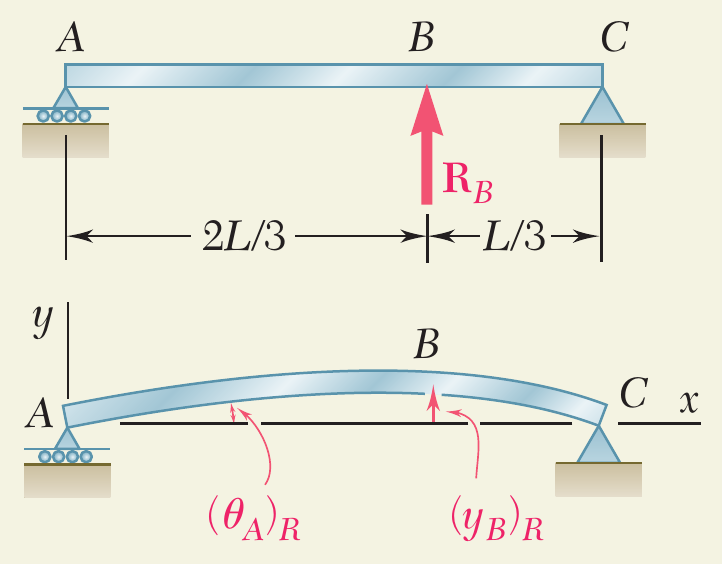
\includegraphics[width=\linewidth,height=2.9cm,keepaspectratio]{Chap_9/sp_9_8_c.png}
  \end{columns}
\end{frame}
% ===========
\begin{frame}[t]{Bài mẫu 9.8 (tiếp)}
  \begin{columns}[T]
    \column{0.56\textwidth}
      \small
      \begin{itemize}
        \setlength{\itemsep}{0.6em}
        \item Để tương thích với các gối ban đầu, $y_B = 0$:
        \[
          0 = (y_B)_w + (y_B)_R = -0{,}01132\frac{wL^4}{EI}
            + 0{,}01646\frac{R_BL^3}{EI}
        \]
        \[
          \boxed{R_B = 0{,}688wL\uparrow}
        \]
        \item Từ tĩnh học:
        \[
          \boxed{R_A = 0{,}271wL\uparrow \qquad R_C = 0{,}0413wL\uparrow}
        \]
      \end{itemize}
    \column{0.42\textwidth}
      \centering
      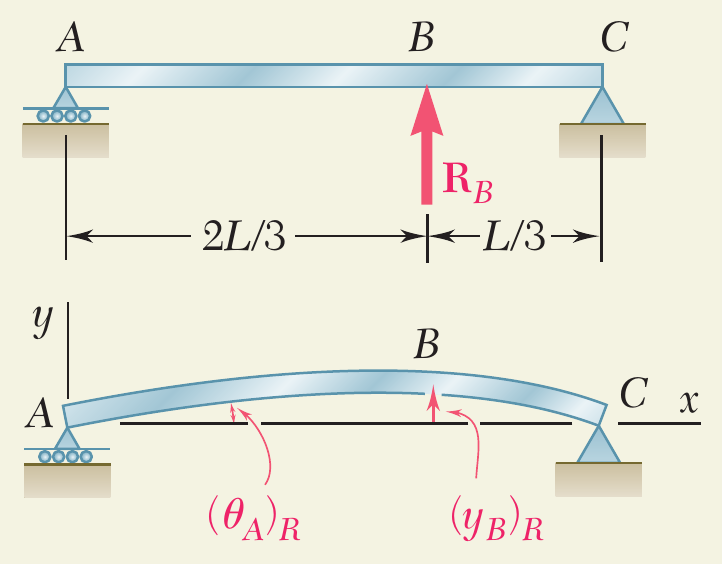
\includegraphics[width=\linewidth,height=5.5cm,keepaspectratio]{Chap_9/sp_9_8_c.png}
  \end{columns}
\end{frame}
% ===========
\begin{frame}[t]{Bài mẫu 9.8 (tiếp)}
  \begin{columns}[T]
    \column{0.58\textwidth}
      \small
      \[
        (\theta_A)_w = -\frac{wL^3}{24EI} = -0{,}04167\frac{wL^3}{EI}
      \]
      \[
        (\theta_A)_R = \frac{Pb(L^2 - b^2)}{6EIL}
          = \frac{0{,}688wL}{6EIL}\left(\frac{L}{3}\right)
            \left[L^2 - \left(\frac{L}{3}\right)^2\right]
      \]
      \[
        (\theta_A)_R = 0{,}03398\frac{wL^3}{EI}
      \]
      Góc xoay tại đầu $A$:
      \[
        \theta_A = (\theta_A)_w + (\theta_A)_R
          = -0{,}04167\frac{wL^3}{EI} + 0{,}03398\frac{wL^3}{EI}
      \]
      \[
        \boxed{\theta_A = -0{,}00769\frac{wL^3}{EI}}
      \]
    \column{0.40\textwidth}
      \centering
      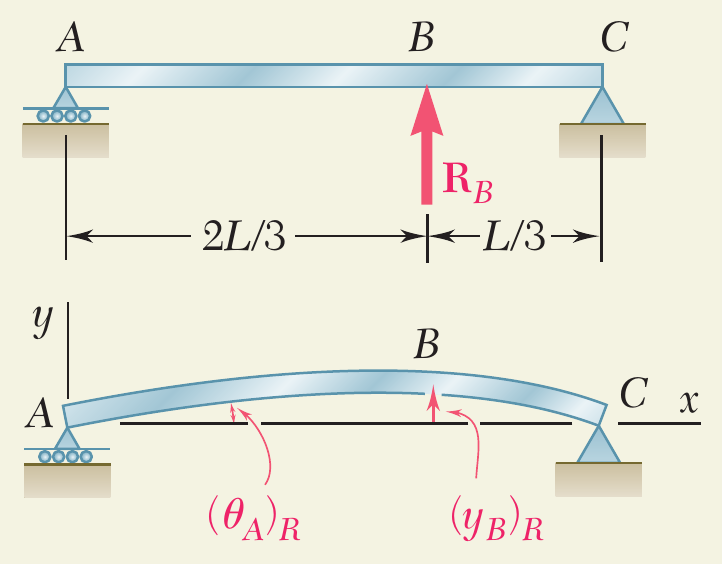
\includegraphics[width=\linewidth,height=5.5cm,keepaspectratio]{Chap_9/sp_9_8_c.png}
  \end{columns}
\end{frame}
% ===========
\section{Các định lý diện tích mô men}
\begin{frame}[t]{Các định lý diện tích mô men}
  \begin{columns}[T]
    \column{0.58\textwidth}
      \small
      \begin{itemize}
        \setlength{\itemsep}{0.5em}
        \item Các tính chất hình học của đường đàn hồi có thể được dùng để xác
              định độ võng và góc xoay.
        \item Xét dầm chịu tải trọng bất kỳ:
        \[
          \frac{d\theta}{dx} = \frac{d^2y}{dx^2} = \frac{M}{EI}
        \]
        \[
          \int_{\theta_C}^{\theta_D}d\theta = \int_{x_C}^{x_D}\frac{M}{EI}\,dx
        \]
        \[
          \theta_D - \theta_C = \int_{x_C}^{x_D}\frac{M}{EI}\,dx
        \]
        \item \textbf{Định lý diện tích mô men thứ nhất:}\\
              $\theta_{D/C}$ = diện tích dưới biểu đồ $(M/EI)$ giữa $C$ và $D$.
      \end{itemize}
    \column{0.40\textwidth}
      \centering
      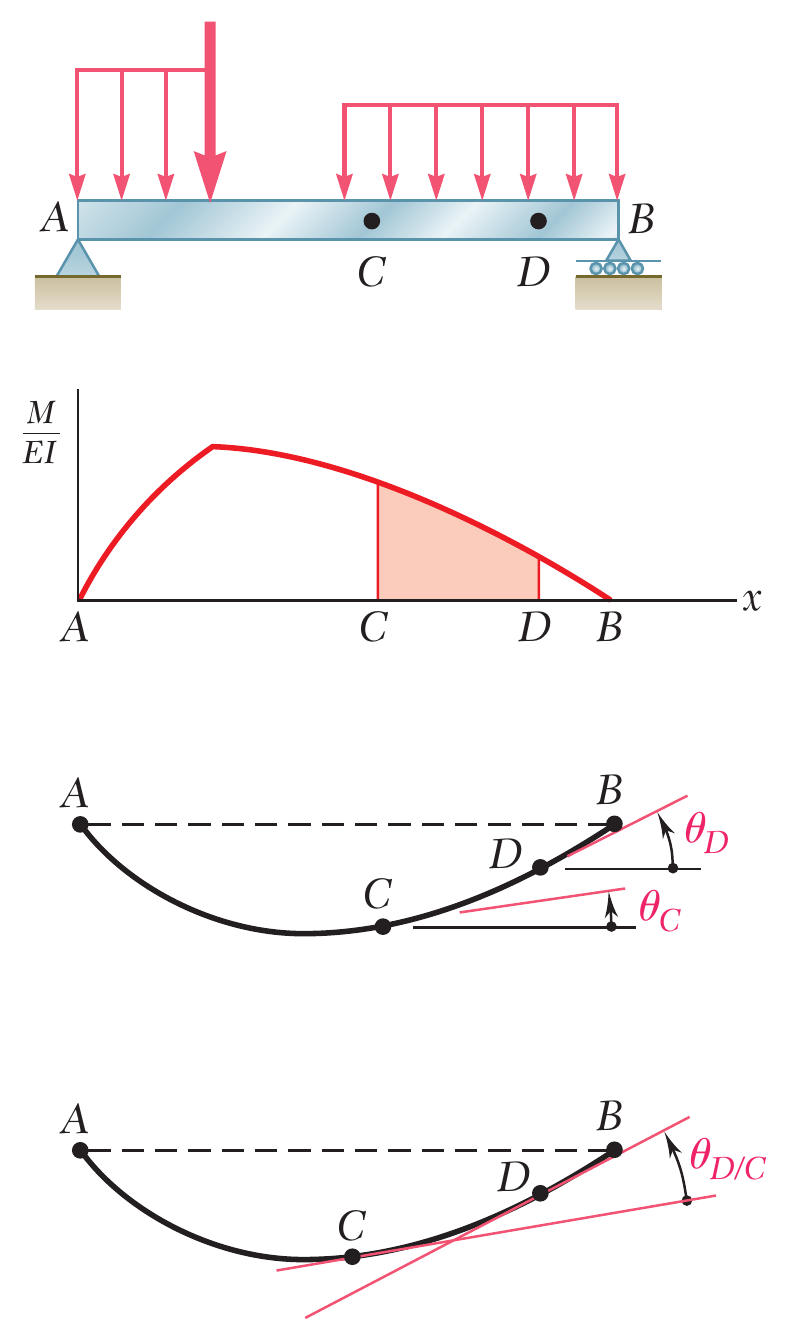
\includegraphics[width=\linewidth,height=1.9cm,keepaspectratio]{Chap_9/fig_9_37.png}\\[2pt]
      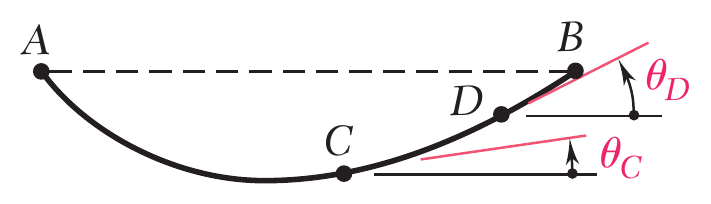
\includegraphics[width=\linewidth,height=1.9cm,keepaspectratio]{Chap_9/fig_9_37_detail.png}\\[2pt]
      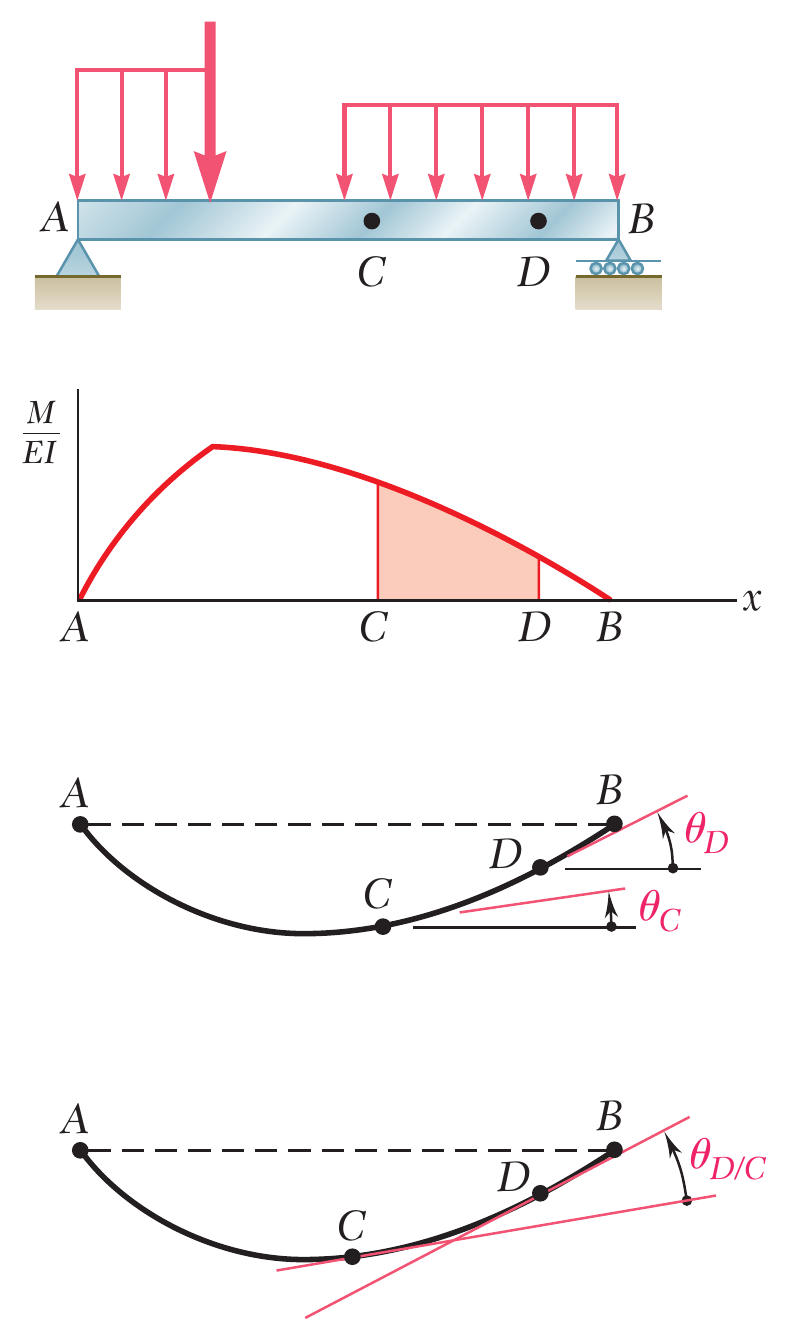
\includegraphics[width=\linewidth,height=1.9cm,keepaspectratio]{Chap_9/fig_9_37.png}
  \end{columns}
\end{frame}
% ===========
\begin{frame}[t]{Các định lý diện tích mô men (tiếp)}
  \begin{columns}[T]
    \column{0.58\textwidth}
      \small
      \begin{itemize}
        \setlength{\itemsep}{0.5em}
        \item Các tiếp tuyến với đường đàn hồi tại $P$ và $P'$ chắn một đoạn
              có chiều dài $dt$ trên đường thẳng đứng qua $C$:
        \[
          dt = x_1\,d\theta = x_1\frac{M}{EI}\,dx
        \]
        \[
          t_{C/D} = \int_{x_C}^{x_D}x_1\frac{M}{EI}\,dx
            = \text{độ lệch tiếp tuyến của } C \text{ đối với } D
        \]
        \item \textbf{Định lý diện tích mô men thứ hai:}\\
              Độ lệch tiếp tuyến của $C$ đối với $D$ bằng mô men tĩnh, đối với
              trục thẳng đứng đi qua $C$, của diện tích dưới biểu đồ $(M/EI)$
              giữa $C$ và $D$.
      \end{itemize}
    \column{0.40\textwidth}
      \centering
      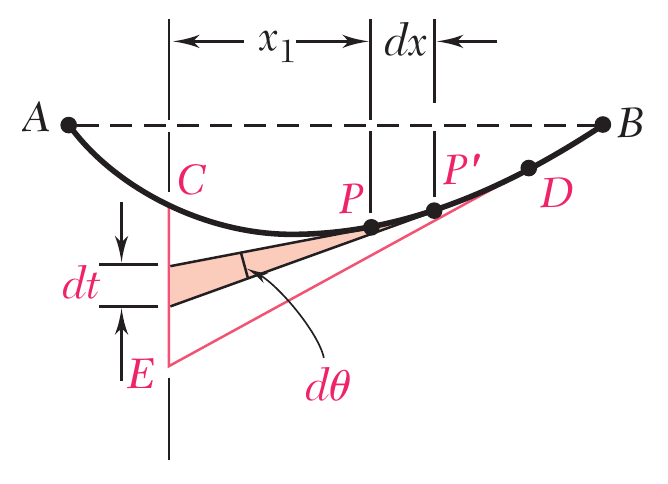
\includegraphics[width=\linewidth,height=2.9cm,keepaspectratio]{Chap_9/fig_9_39.png}\\[2pt]
      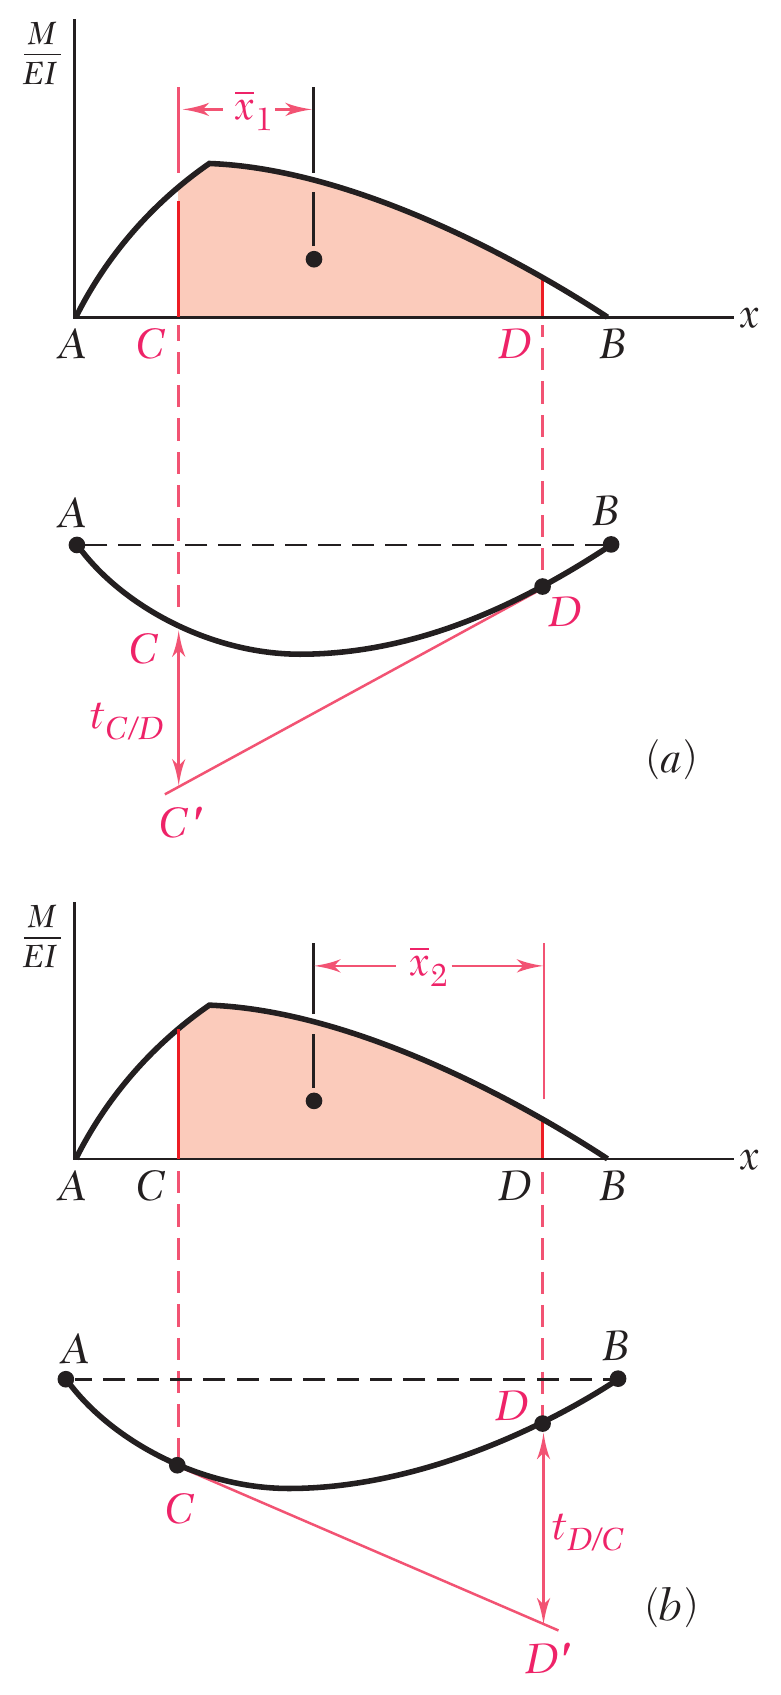
\includegraphics[width=\linewidth,height=2.9cm,keepaspectratio]{Chap_9/fig_9_41.png}
  \end{columns}
\end{frame}
% ===========
\section{Áp dụng cho dầm công xôn và dầm chịu tải đối xứng}
\begin{frame}[t]{Áp dụng cho dầm công xôn và dầm chịu tải đối xứng}
  \begin{columns}[T]
    \column{0.56\textwidth}
      \small
      \begin{itemize}
        \setlength{\itemsep}{0.8em}
        \item \textbf{Dầm công xôn} -- chọn tiếp tuyến tại $A$ làm tiếp tuyến
              tham chiếu. Với $\theta_A = 0$:
        \[
          \theta_D = \theta_{D/A} \qquad y_D = t_{D/A}
        \]
        \item \textbf{Dầm tựa đơn chịu tải đối xứng} -- chọn tiếp tuyến tại
              $C$ làm tiếp tuyến tham chiếu. Với $\theta_C = 0$:
        \[
          \theta_B = \theta_{B/C} \qquad y_B = t_{B/C}
        \]
      \end{itemize}
    \column{0.42\textwidth}
      \centering
      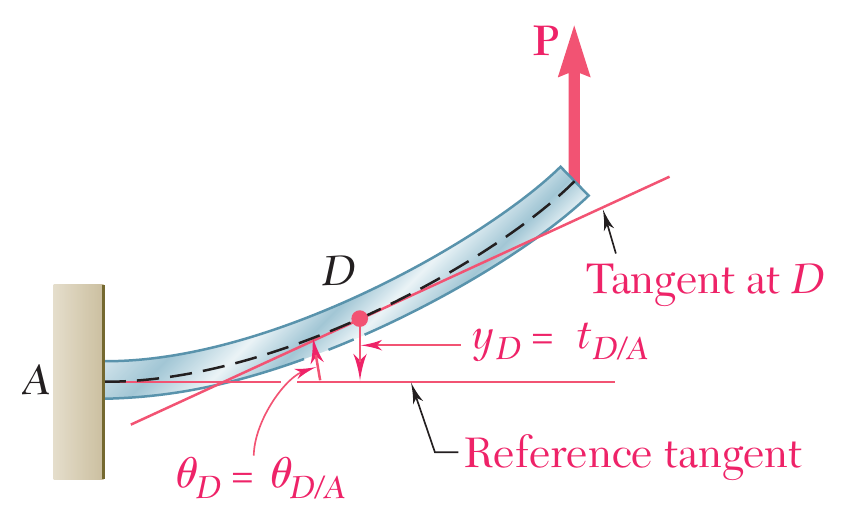
\includegraphics[width=\linewidth,height=1.9cm,keepaspectratio]{Chap_9/fig_9_42.png}\\[2pt]
      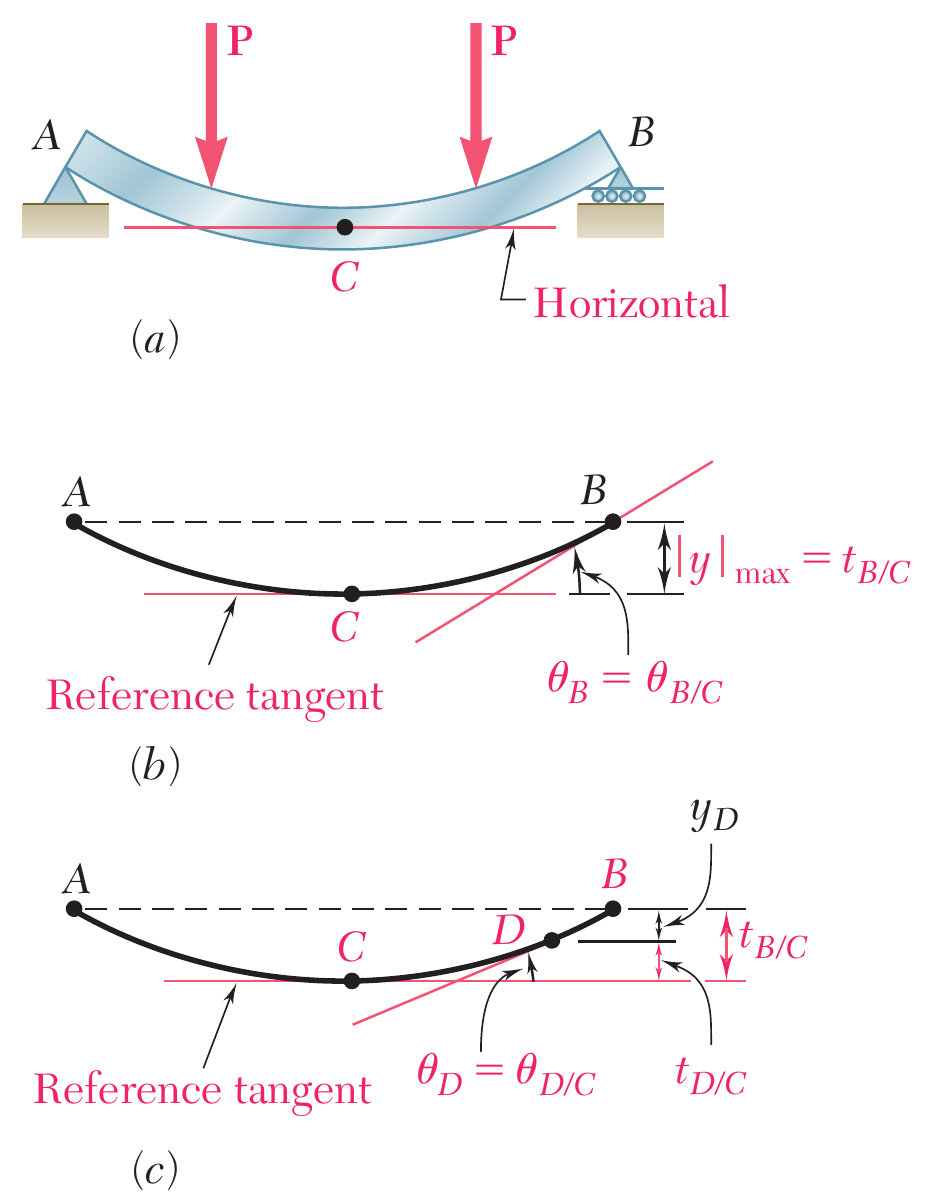
\includegraphics[width=\linewidth,height=1.9cm,keepaspectratio]{Chap_9/fig_9_43.png}\\[2pt]
      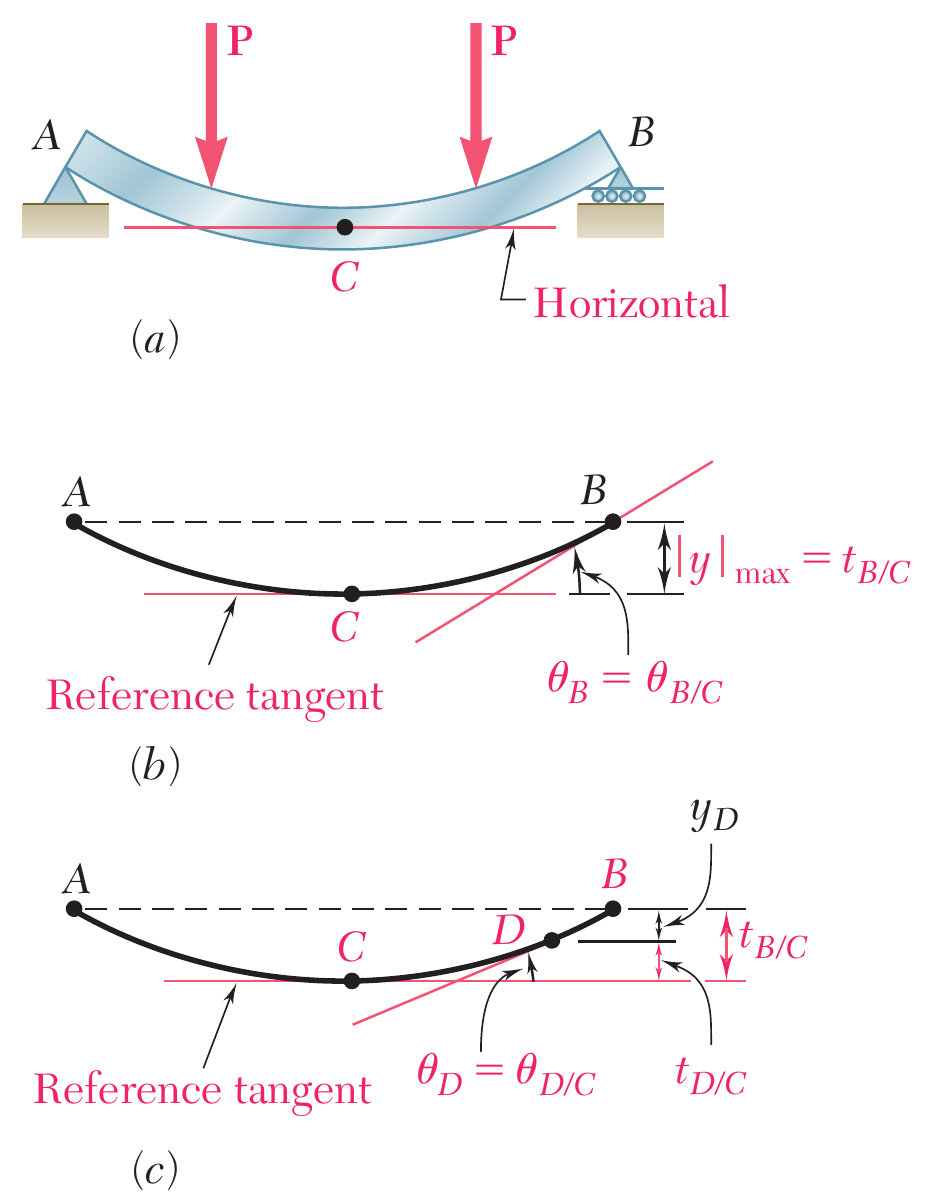
\includegraphics[width=\linewidth,height=1.9cm,keepaspectratio]{Chap_9/fig_9_43.png}
  \end{columns}
\end{frame}
% ===========
\section{Vẽ biểu đồ mô men uốn theo từng phần}
\begin{frame}[t]{Vẽ biểu đồ mô men uốn theo từng phần}
  \begin{columns}[T]
    \column{0.58\textwidth}
      \small
      \begin{itemize}
        \setlength{\itemsep}{0.5em}
        \item Việc xác định độ thay đổi góc xoay và độ lệch tiếp tuyến được đơn
              giản hóa nếu ảnh hưởng của từng tải trọng được tính riêng.
        \item Vẽ biểu đồ $(M/EI)$ riêng cho từng tải trọng.
              \begin{itemize}
                \item Độ thay đổi góc xoay $\theta_{D/C}$ nhận được bằng cách
                      cộng các diện tích dưới các biểu đồ.
                \item Độ lệch tiếp tuyến $t_{D/C}$ nhận được bằng cách cộng mô
                      men tĩnh của các diện tích đối với trục thẳng đứng qua
                      $D$.
              \end{itemize}
        \item Biểu đồ mô men uốn được vẽ từ các tải trọng riêng rẽ được gọi là
              biểu đồ vẽ \emph{theo từng phần}.
      \end{itemize}
    \column{0.40\textwidth}
      \centering
      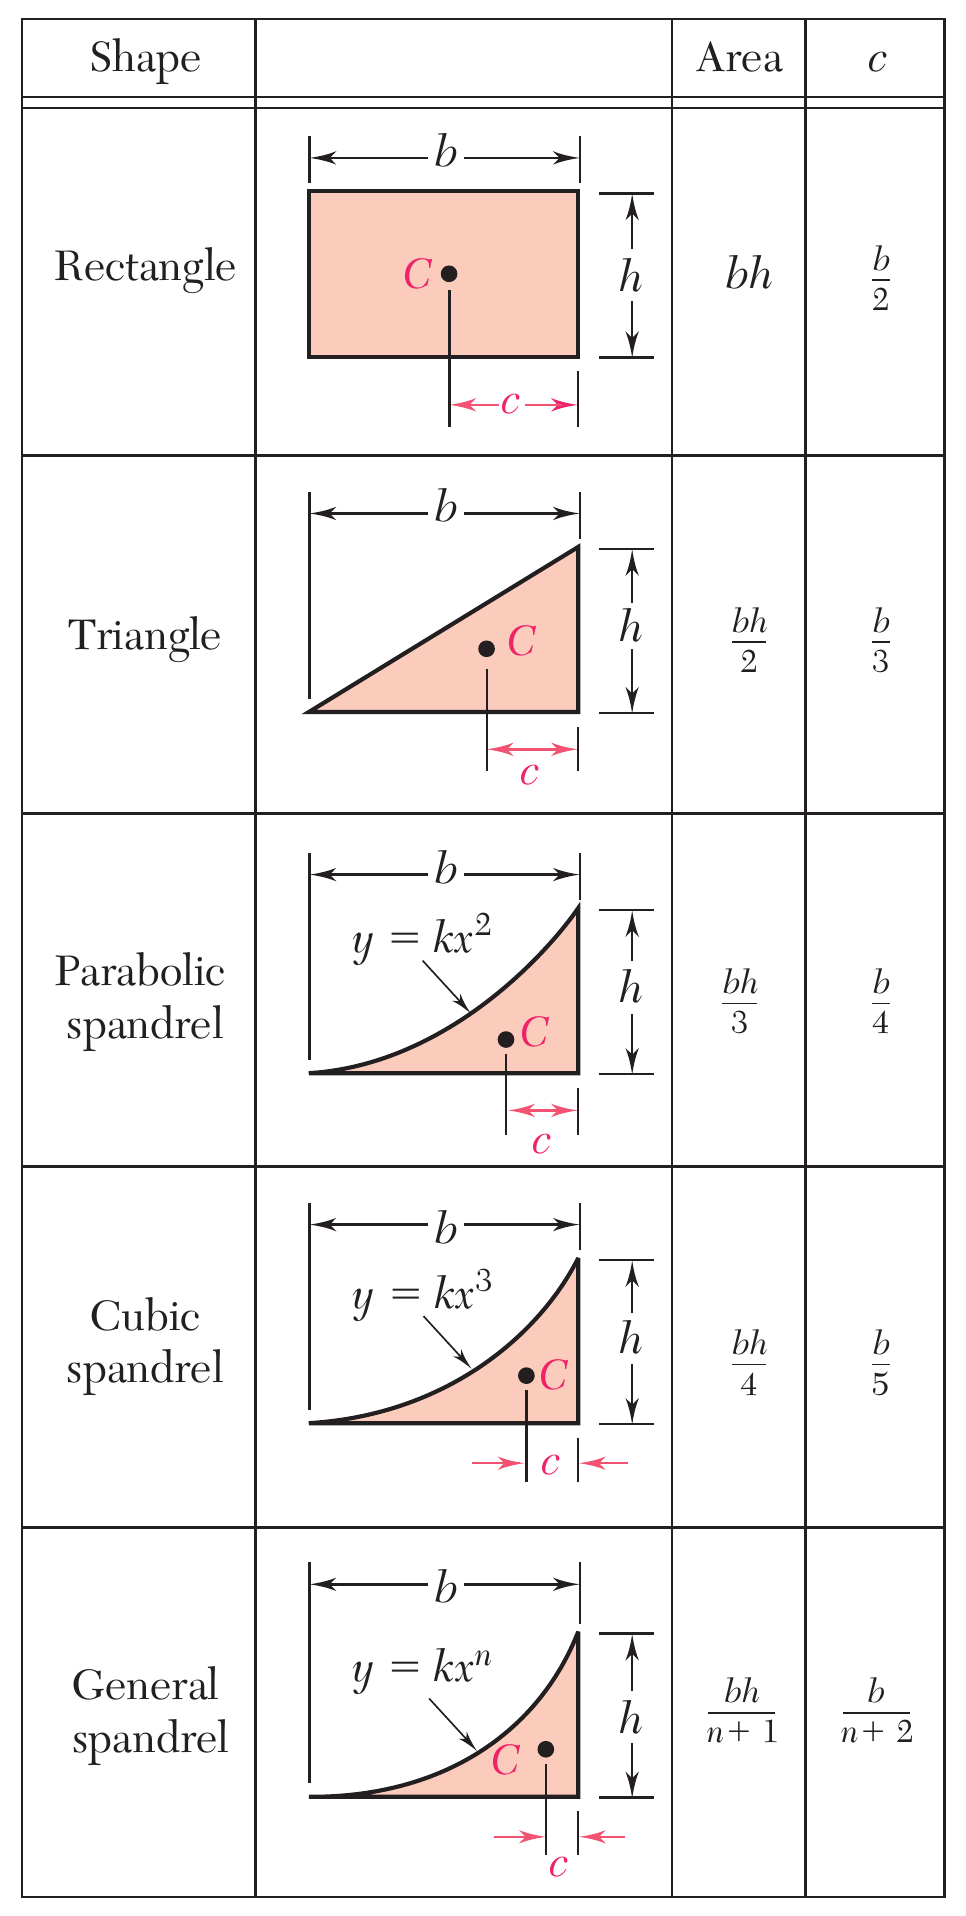
\includegraphics[width=\linewidth,height=5.5cm,keepaspectratio]{Chap_9/fig_9_48.png}
  \end{columns}
\end{frame}
% ===========
\section{Bài mẫu 9.11}
\begin{frame}[t]{Bài mẫu 9.11}
  \begin{columns}[T]
    \column{0.42\textwidth}
      \centering
      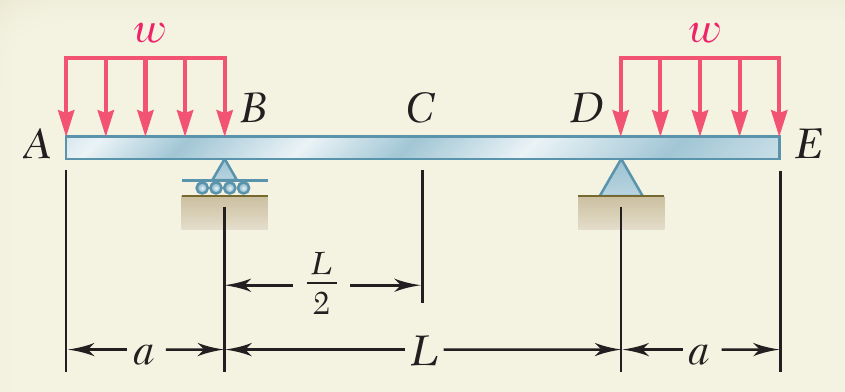
\includegraphics[width=\linewidth,height=5.5cm,keepaspectratio]{Chap_9/sp_9_11_a.png}
    \column{0.56\textwidth}
      \small
      Với dầm lăng trụ như hình vẽ, xác định góc xoay và độ võng tại $E$.

      \vspace{0.8em}
      \textbf{LỜI GIẢI:}
      \begin{itemize}
        \setlength{\itemsep}{0.5em}
        \item Xác định phản lực tại các gối.
        \item Vẽ các biểu đồ lực cắt, mô men uốn và $(M/EI)$.
        \item Lấy tiếp tuyến tại $C$ làm tiếp tuyến tham chiếu, tính góc xoay
              và các độ lệch tiếp tuyến tại $E$.
      \end{itemize}
  \end{columns}
\end{frame}
% ===========
\begin{frame}[t]{Bài mẫu 9.11 (tiếp)}
  \begin{columns}[T]
    \column{0.52\textwidth}
      \small
      \textbf{LỜI GIẢI:}
      \begin{itemize}
        \setlength{\itemsep}{0.5em}
        \item Xác định phản lực tại các gối:
        \[
          R_B = R_D = wa
        \]
        \item Vẽ các biểu đồ lực cắt, mô men uốn và $(M/EI)$:
        \[
          A_1 = -\frac{wa^2}{2EI}\left(\frac{L}{2}\right) = -\frac{wa^2L}{4EI}
        \]
        \[
          A_2 = -\frac{1}{3}\left(\frac{wa^2}{2EI}\right)(a) = -\frac{wa^3}{6EI}
        \]
      \end{itemize}
    \column{0.46\textwidth}
      \centering
      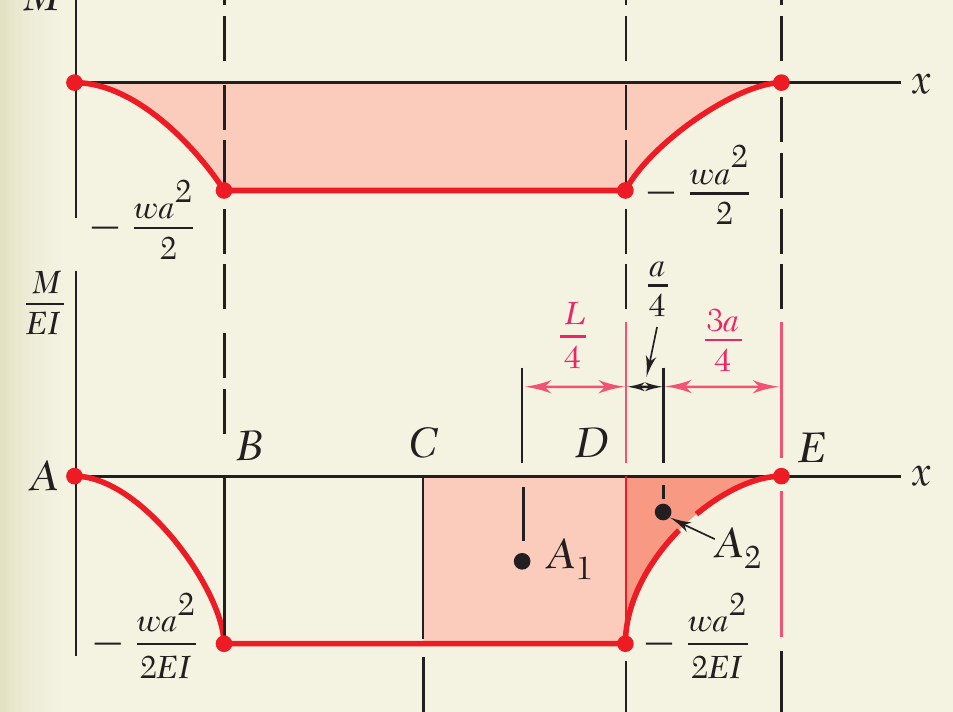
\includegraphics[width=\linewidth,height=5.5cm,keepaspectratio]{Chap_9/sp_9_11_b.png}
  \end{columns}
\end{frame}
% ===========
\begin{frame}[t]{Bài mẫu 9.11 (tiếp)}
  \begin{columns}[T]
    \column{0.60\textwidth}
      \footnotesize
      \begin{itemize}
        \setlength{\itemsep}{0.20em}
        \item Góc xoay tại $E$:
        \[
          \theta_E = \theta_C + \theta_{E/C} = \theta_{E/C}
            = A_1 + A_2 = -\frac{wa^2L}{4EI} - \frac{wa^3}{6EI}
        \]
        \[
          \boxed{\theta_E = -\frac{wa^2}{12EI}(3L + 2a)}
        \]
        \item Độ võng tại $E$:
        \[
          y_E = t_{E/C} - t_{D/C}
        \]
        \[
          = \left[A_1\left(a + \frac{L}{4}\right) + A_2\left(\frac{3a}{4}\right)\right]
              - \left[A_1\left(\frac{L}{4}\right)\right]
        \]
        \[
          = A_1a + A_2\left(\frac{3a}{4}\right)
            = -\frac{wa^3L}{4EI} - \frac{wa^4}{8EI}
        \]
        \[
          \boxed{y_E = -\frac{wa^3}{8EI}(2L + a)}
        \]
      \end{itemize}
    \column{0.38\textwidth}
      \centering
      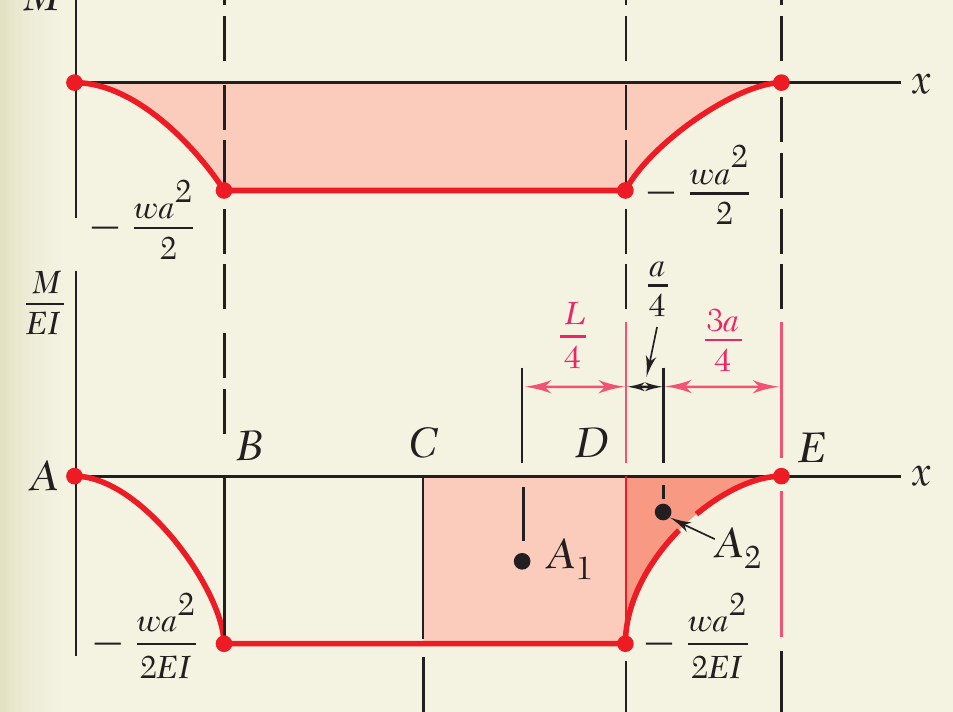
\includegraphics[width=\linewidth,height=2.5cm,keepaspectratio]{Chap_9/sp_9_11_b.png}\\[2pt]
      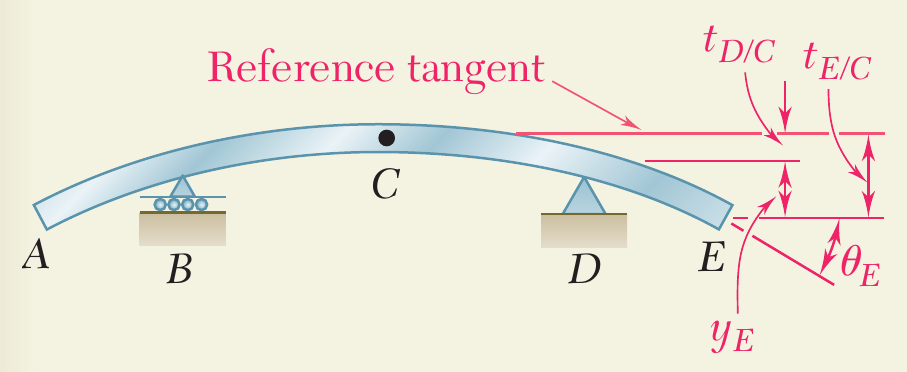
\includegraphics[width=\linewidth,height=2.5cm,keepaspectratio]{Chap_9/sp_9_11_c.png}
  \end{columns}
\end{frame}
% ===========
\section{Áp dụng cho dầm chịu tải không đối xứng}
\begin{frame}[t]{Áp dụng định lý diện tích mô men cho dầm chịu tải không đối xứng}
  \begin{columns}[T]
    \column{0.58\textwidth}
      \small
      \begin{itemize}
        \setlength{\itemsep}{0.5em}
        \item Chọn tiếp tuyến tham chiếu tại gối $A$. Tính $\theta_A$ bằng cách
              xác định độ lệch tiếp tuyến tại $B$ đối với $A$:
        \[
          \theta_A = -\frac{t_{B/A}}{L}
        \]
        \item Góc xoay tại các điểm khác được tìm đối với tiếp tuyến tham chiếu:
        \[
          \theta_D = \theta_A + \theta_{D/A}
        \]
        \item Độ võng tại $D$ được tìm từ độ lệch tiếp tuyến tại $D$:
        \[
          \frac{EF}{x} = \frac{HB}{L} \qquad EF = \frac{x}{L}t_{B/A}
        \]
        \[
          y_D = ED - EF = t_{D/A} - \frac{x}{L}t_{B/A}
        \]
      \end{itemize}
    \column{0.40\textwidth}
      \centering
      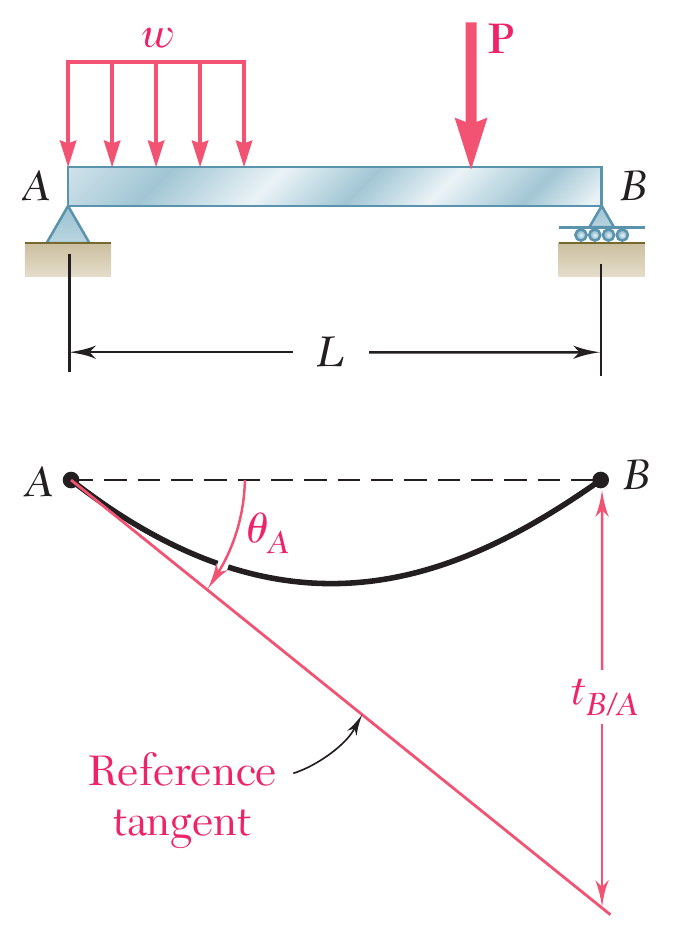
\includegraphics[width=\linewidth,height=2.9cm,keepaspectratio]{Chap_9/fig_9_55.png}\\[2pt]
      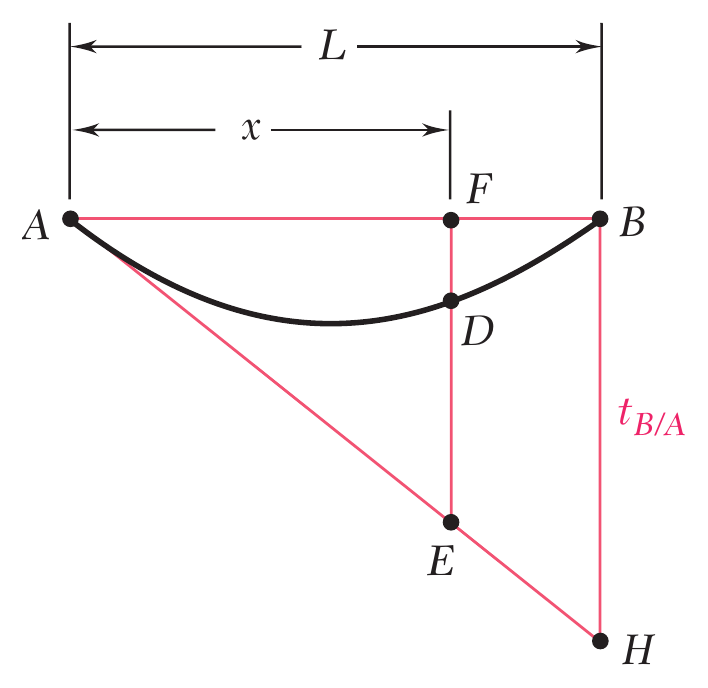
\includegraphics[width=\linewidth,height=2.9cm,keepaspectratio]{Chap_9/fig_9_59.png}
  \end{columns}
\end{frame}
% ===========
\section{Độ võng lớn nhất}
\begin{frame}[t]{Độ võng lớn nhất}
  \begin{columns}[T]
    \column{0.58\textwidth}
      \small
      \begin{itemize}
        \setlength{\itemsep}{0.5em}
        \item Độ võng lớn nhất xảy ra tại điểm $K$, nơi tiếp tuyến nằm ngang:
        \[
          \theta_A = -\frac{t_{B/A}}{L}
        \]
        \[
          \theta_K = 0 = \theta_A + \theta_{K/A}
          \qquad \theta_{K/A} = -\theta_A
        \]
        \item Điểm $K$ có thể xác định bằng cách lấy một diện tích dưới biểu đồ
              $(M/EI)$ bằng $-\theta_A$.
        \item Tìm $y_{\max}$ bằng cách tính mô men tĩnh, đối với trục thẳng
              đứng qua $A$, của diện tích giữa $A$ và $K$.
      \end{itemize}
    \column{0.40\textwidth}
      \centering
      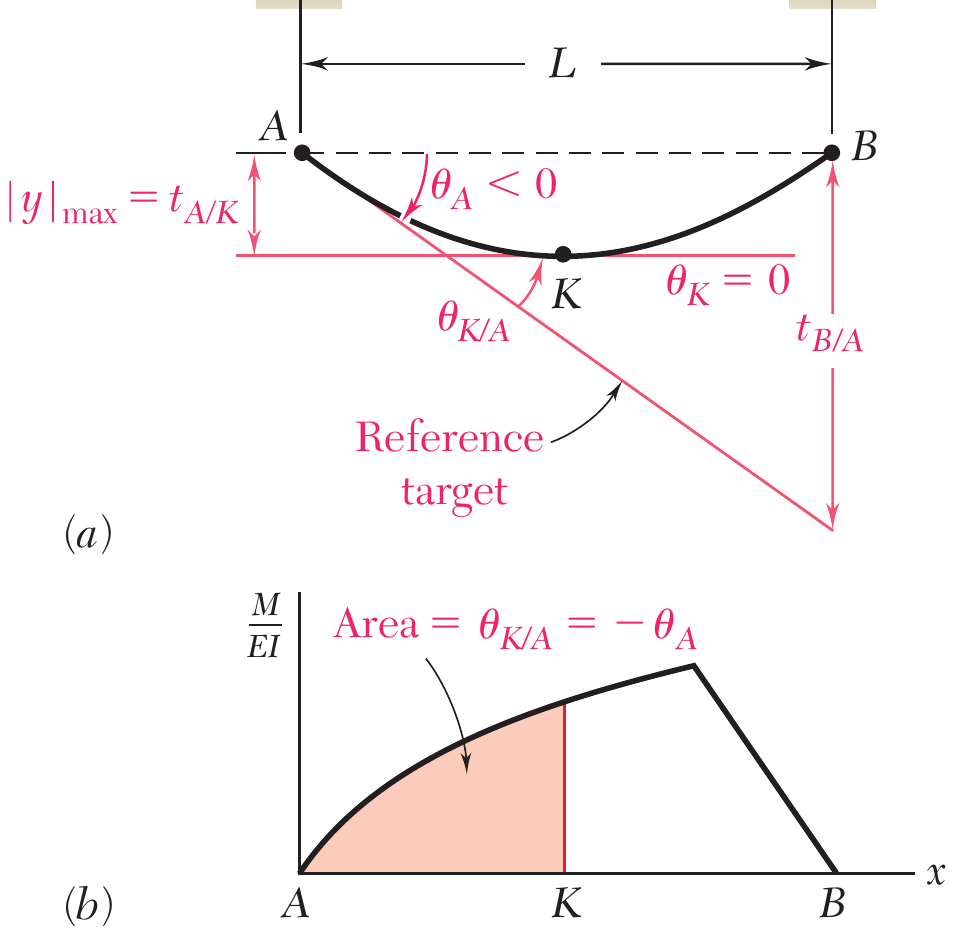
\includegraphics[width=\linewidth,height=2.9cm,keepaspectratio]{Chap_9/fig_9_63.png}\\[2pt]
      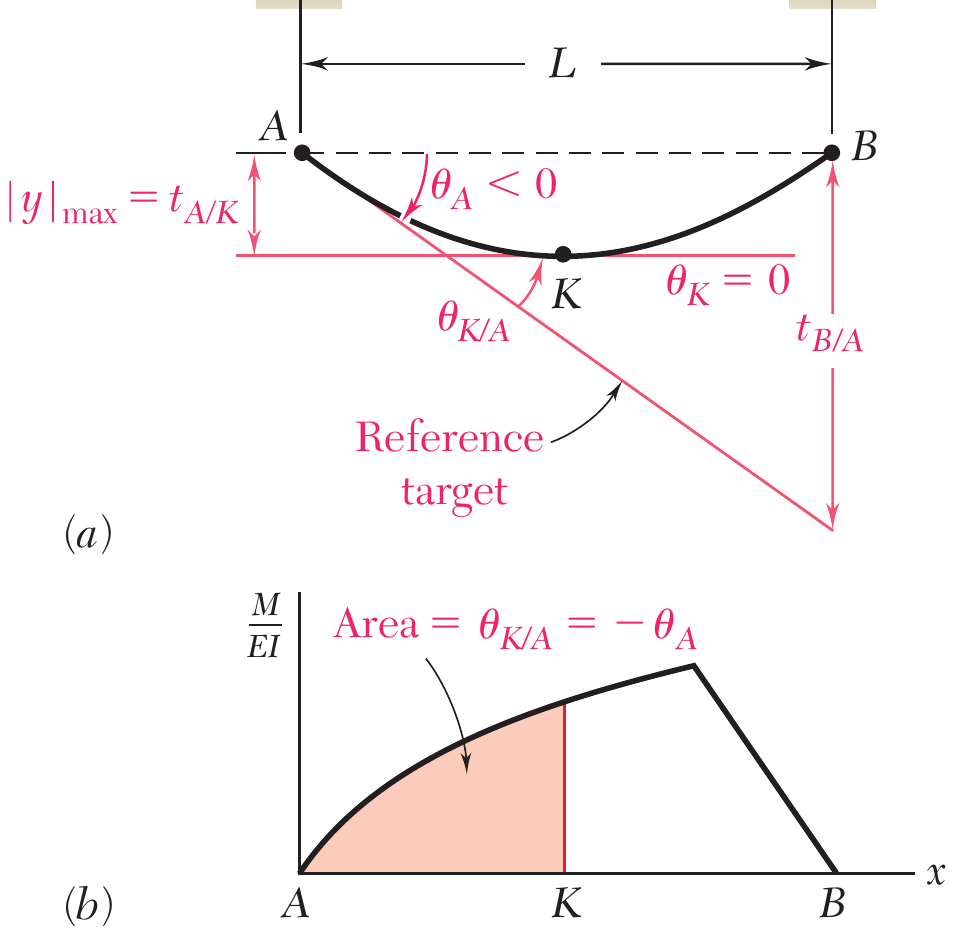
\includegraphics[width=\linewidth,height=2.9cm,keepaspectratio]{Chap_9/fig_9_63.png}
  \end{columns}
\end{frame}
% ===========
\section{Định lý diện tích mô men với dầm siêu tĩnh}
\begin{frame}[t]{Sử dụng định lý diện tích mô men với dầm siêu tĩnh}
  \begin{columns}[T]
    \column{0.58\textwidth}
      \small
      \begin{itemize}
        \setlength{\itemsep}{0.7em}
        \item Phản lực tại các gối của dầm siêu tĩnh được tìm bằng cách chọn
              một liên kết thừa và coi nó là tải trọng chưa biết thỏa mãn điều
              kiện tương thích chuyển vị.
        \item Biểu đồ $(M/EI)$ được vẽ theo từng phần. Các độ lệch tiếp tuyến
              nhận được được cộng tác dụng và liên hệ với nhau bằng điều kiện
              tương thích.
        \item Khi đã xác định được phản lực, góc xoay và độ võng được tìm bằng
              phương pháp diện tích mô men.
      \end{itemize}
    \column{0.40\textwidth}
      \centering
      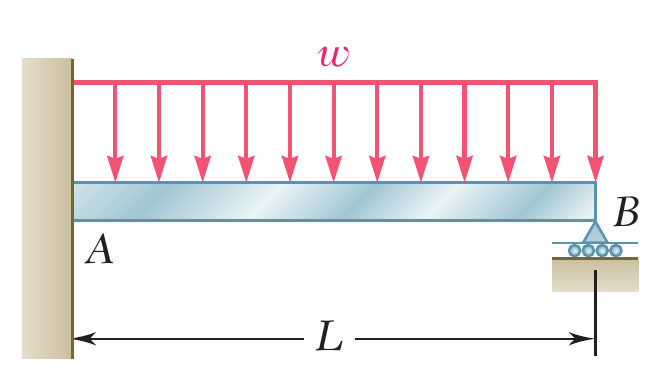
\includegraphics[width=\linewidth,height=2.9cm,keepaspectratio]{Chap_9/fig_9_66.png}\\[2pt]
      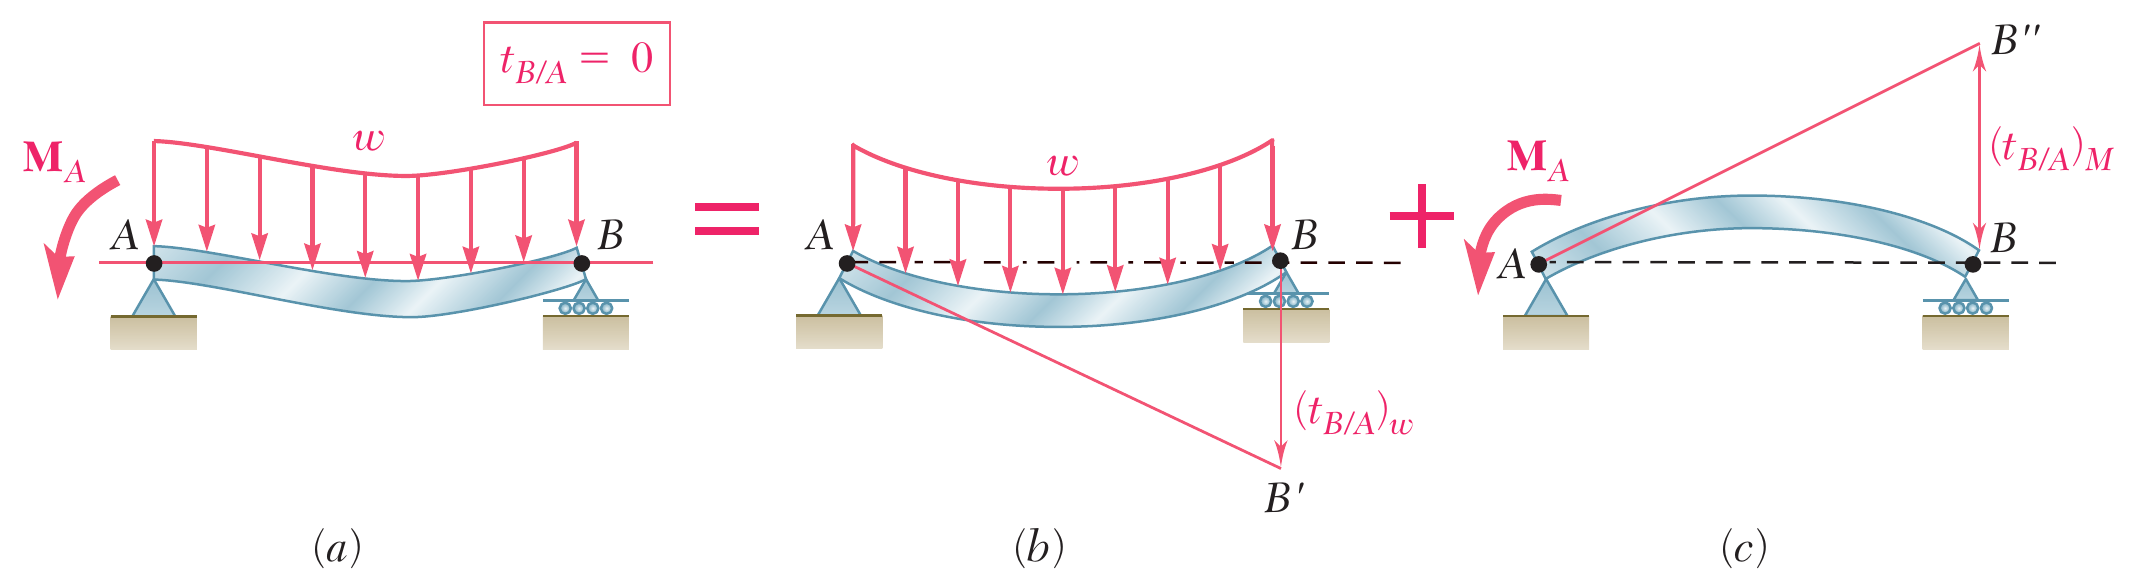
\includegraphics[width=\linewidth,height=2.9cm,keepaspectratio]{Chap_9/fig_9_67.png}
  \end{columns}
\end{frame}

\end{document}
